\documentclass[11pt]{article}

 

 
\usepackage[margin=1.25in]{geometry}
\usepackage[round]{natbib} 
\usepackage[utf8]{inputenc}
\usepackage[T1]{fontenc}
\usepackage{lmodern}
\usepackage{xcolor} 
\definecolor{purple}{RGB}{128,0,128}
\definecolor{gray}{gray}{0.45}

 
\usepackage{amsmath,amssymb,amsthm,mathtools}
\numberwithin{equation}{section}

 
\usepackage{microtype}
\usepackage{graphicx}
 
\usepackage{subcaption}  
\usepackage{booktabs}  
\usepackage{placeins}
 
\graphicspath{{figs/}{figs/cifar10/}{plots/}{results-stressed-cap80/plots/}{paper-extra-experiments/plots/}}

 
\usepackage{enumitem}
\usepackage{listings}

\usepackage{tabularx}
\usepackage{ragged2e}  

 

 
\lstset{
language=Python,
basicstyle=\ttfamily\footnotesize,
breaklines=true,
breakatwhitespace=false,
showstringspaces=false,
captionpos=b,
frame=single,
numbers=left,
numberstyle=\tiny\color{gray},
keywordstyle=\color{blue},
commentstyle=\color{green!60!black},
stringstyle=\color{purple}
}

\usepackage{hyperref} 
\hypersetup{
colorlinks=true,
linkcolor=blue!70!black,
citecolor=blue!70!black,
urlcolor=blue!70!black
}


% --- THEOREMS ---
\theoremstyle{plain}
\newtheorem{theorem}{Theorem}[section]
\newtheorem{proposition}[theorem]{Proposition}
\newtheorem{corollary}[theorem]{Corollary}
\newtheorem{lemma}[theorem]{Lemma}
\newtheorem{assumption}[theorem]{Assumption}
\newtheorem{fact}[theorem]{Fact}
\newtheorem{claim}[theorem]{Claim}

\theoremstyle{definition}
\newtheorem{definition}[theorem]{Definition}

\theoremstyle{remark}
\newtheorem{remark}[theorem]{Remark}


% --- MACROS ---
\newcommand{\R}{\mathbb{R}}
\newcommand{\e}{\mathrm{e}}
\newcommand{\ones}{\mathbf{1}}
\newcommand{\cB}{\mathcal{B}}
\newcommand{\cP}{\mathcal{P}}
\newcommand{\diag}{\operatorname{diag}}
\newcommand{\tr}{\operatorname{Tr}}
\newcommand{\ip}[2]{\left\langle #1, #2 \right\rangle}
\newcommand{\norm}[1]{\left\lVert #1 \right\rVert}
\newcommand{\abs}[1]{\left\lvert #1 \right\rvert}
\newcommand{\Hres}{H_{\mathrm{res}}}
\newcommand{\Hpre}{H_{\mathrm{pre}}}
\newcommand{\Hpost}{H_{\mathrm{post}}}
\newcommand{\KL}{\operatorname{KL}}
\newcommand{\Ent}{\operatorname{Ent}} 
\newcommand{\vecop}{\operatorname{vec}}
\newcommand{\Amax}{\textsf{Amax}\,}
\newcommand{\kobs}{\kappa_{\mathrm{obs}}}
\newcommand{\epstol}{\varepsilon_{\mathrm{tol}}}
\newcommand{\epsfloor}{\varepsilon_{\mathrm{floor}}}
\newcommand{\tstop}{t_{\mathrm{stop}}}
\newcommand{\tmax}{t_{\max}}

\title{Finite-Step Sinkhorn Certificates for Nonnegative Stream-Mixing Products}


\author{Maksim Kosmakov}

\date{}

\begin{document}
\maketitle
 
\begin{abstract}
We give deterministic finite-step Sinkhorn certificates for the nonnegative
stream-mixing pathway in expanded-stream residual architectures, motivated by
Manifold-Constrained Hyper-Connections (mHC).  The central object is the
depth-wise mixer product
\[
        T_L=H_{\rm res}^{(L)}H_{\rm res}^{(L-1)}\cdots H_{\rm res}^{(1)} ,
\]
not an unconditional stability theorem for the full nonlinear network.

For entrywise nonnegative mixers, row and column marginal errors are induced-norm
certificates: they bound the forward $\ell_\infty$ and backward $\ell_1$
streamwise \(A_{\max}\) gains.  Thus finite Sinkhorn steps give a theorem chain
\[
    \varepsilon_c^{(\ell)}
    \Rightarrow
    \|H_{\rm res}^{(\ell)}\|_1\le 1+\varepsilon_c^{(\ell)}
    \Rightarrow
    \|T_L\|_1\le \prod_{\ell=1}^L(1+\varepsilon_c^{(\ell)}).
\]
For the \texttt{column-then-row} normalization order considered here, we prove a
Hilbert-projective finite-step bound with the correct half-step loss for the
output column error.  This maps logit dynamic range and Sinkhorn step budget to
a certified depth-wise backward budget for the mixer product.

We also separate certificates from predictors.  Worst-case Hilbert bounds are
safe but pessimistic; near the Sinkhorn limit, the sharp local full-step rate is
\(\sigma_2(P)^2\), where \(P\) is the limiting doubly stochastic scaling.  We
state a conditional local derivative-envelope certificate and first-/second-order
finite-step predictors for interpreting observed decay curves.  The numerical
section is diagnostic: it reports achieved marginal errors, product certificates,
exact realized backward gains by vector propagation, cap failures, and the gap
between worst-case certificates and local predictors.
\end{abstract}












\section{Introduction}\label{sec:intro}

Deep neural networks rely on controlled signal propagation to avoid vanishing or exploding gradients. Standard stabilizers
such as normalization layers, e.g.\ LayerNorm~\citep{Ba2016LayerNorm}, and careful initialization reduce feature-scale drift, but they do not directly
constrain another source of instability that appears in expanded-stream architectures: \emph{products of stream-mixing matrices}
across depth. Related work includes stability-motivated architectures \citep{HaberRuthotto2018} and continuous-depth viewpoints \citep{Chen2018NeuralODE}.

In expanded-stream residual designs, each layer introduces a mixer $\Hres^{(\ell)}\in\R^{n\times n}$ that routes information across
$n$ parallel streams.\footnote{Throughout, the row index is the \emph{stream} index (not batch); batch is treated as an outer dimension and omitted from notation.}
If the depth-wise product of these mixers has a large induced norm, signals (and, in backpropagation, gradients) can be amplified through the mixing pathway even when per-feature normalization is present.

Row-stochasticity alone does not control the backward mixing-path gain. For any $n\ge 2$, the row-stochastic matrix
$H=\ones \mathbf{e}_1^\top$ satisfies $\|H\|_\infty=1$ but has column sum $n$ in the first column, hence $\|H\|_1=n$.
Thus, row-only normalization can induce backward amplification on the order of the expansion rate.
Finite-step Sinkhorn targets both marginals; we quantify how many Sinkhorn steps suffice to certify a prescribed depth-$L$ backward budget.

The motivating architecture class is Manifold-Constrained Hyper-Connections (mHC), which enforce entrywise nonnegativity and drive mixers toward the Birkhoff polytope of doubly stochastic matrices. Since exact projection is computationally expensive, the mHC-motivated mixer parameterization considered here
exponentiates logits to enforce strict positivity and then applies a \emph{finite} number of Sinkhorn--Knopp normalizations \citep{SinkhornKnopp1967,Knight2008}, creating a gap
between the ideal (exact marginals) and the realized finite-step mixers. This paper addresses the corresponding calibration task:
given depth $L$ and a target backward budget $B_1$ for the mixing pathway (i.e., $\|T_L\|_1\le B_1$), we give a conservative rule that maps
(i) logit range/temperature (dynamic range $\kappa$) and (ii) a finite Sinkhorn step budget $t_{\max}$ to a certified column-marginal tolerance that is sufficient to guarantee the depth-$L$ budget \emph{during training}.

\medskip
The practical output is not only a post-hoc bound, but a controller for finite-step normalization. Given a target budget $B_1$, the theory gives: an adaptive stopping rule that redistributes the remaining log-budget across layers; a temperature--clipping condition that translates $(\beta,R,t_{\max})$ into a guaranteed tolerance; a certificate-aware regularizer that can be added to the training objective; and an exact realized backward-gain diagnostic computed by a single vector propagation. Thus the number of Sinkhorn steps is tied to a verifiable stability budget rather than treated only as a heuristic hyperparameter.

\medskip
Sinkhorn--Knopp scaling and matrix balancing are classical \citep{SinkhornKnopp1967,FranklinLorenz1989,Knight2008}, and Hilbert’s projective metric provides a standard contraction framework for positive maps \citep{Birkhoff1957,Bushell1973}.
In machine learning, Sinkhorn iterations are a standard primitive for entropic regularized optimal transport and ``Sinkhorn distances'' \citep{Cuturi2013,PeyreCuturi2019}, and doubly-stochastic attention has been pursued via Sinkhorn-style normalization \citep{Sander2022Sinkformers} and alternative objectives \citep{Shahbazi2025ESPFormer}. 
Prior work often uses Sinkhorn normalization as a layer or operator; here we
certify the finite-step normalization error needed to control the depth-wise
product of nonnegative stream mixers.

In this paper we analyze the \emph{finite-step} normalization regime in residual backbones and derive deterministic worst-case certificates for depth-wise products of mixers. To keep the guarantees aligned with the mixing pathway in backpropagation, we phrase them in terms of coordinate-wise max-norm (\Amax) amplification.\phantomsection\label{subsec:intro_amax}
 Because backpropagation through the mixing map applies $H^\top$,
the induced norms $\|\cdot\|_\infty$ (forward) and $\|\cdot\|_1$ (backward) provide the natural worst-case guarantees for this diagnostic.
Spectral-norm control would require norm conversions (e.g., $\|v\|_2\le \sqrt{n}\|v\|_\infty$) that introduce dimension factors and obscure depth-wise budgets.
For depth $L$, define the composite mixer
\begin{equation}\label{eq:TLdef}
T_L := \Hres^{(L)}\Hres^{(L-1)}\cdots \Hres^{(1)}.
\end{equation}
In the idealized \texttt{column-then-row} normalization order considered here, the output has exact row sums; in implementations with denominator stabilizers the row defect is measured explicitly and is negligible in the reported runs. Thus, for the idealized nonnegative mixer $H\ge 0$ one has $\|H\|_\infty=1$, and the remaining design question is control of the backward gain via $\|T_L\|_1$ (Lemma~\ref{lem:output_rows_exact} and Remark~\ref{rem:additive-stabilizers}).

\paragraph{Scope of the guarantees.}
The certificates in this paper are mixer-path certificates.  More precisely,
they control the depth-wise product \(T_L\) in the induced \(\ell_\infty\) and
\(\ell_1\) matrix norms, equivalently in the forward and backward streamwise
\Amax gains of the residual mixing pathway.  They should not be read as
unconditional end-to-end stability theorems for the full neural network.  When
the nonlinear residual branch is included, one also needs independent bounds,
estimates, or regularization of the corresponding branch Jacobians.  We record
such a composition bound below, but the main deterministic contribution is the
finite-step certificate for the nonnegative Sinkhorn-normalized mixer product.

\paragraph{What is not claimed.}
We do not claim state-of-the-art empirical accuracy, nor do we prove
unconditional full-network stability.  The deterministic guarantee is for the
nonnegative stream-mixing product produced by finite-step Sinkhorn
normalization.  The experiments are therefore reported as numerical diagnostics
for the certificate mechanism rather than as a broad benchmark study.

\paragraph{Contributions.}\label{subsec:intro_contrib}
\begin{itemize}[leftmargin=*, itemsep=0.25em]
\item \textbf{Mixer-product \Amax certificates from marginal errors.}
For entrywise nonnegative mixers, row and column marginal errors directly
control \(\|H\|_\infty\) and \(\|H\|_1\), giving depth-wise forward and
backward \Amax budgets for \(T_L\) (Theorem~\ref{prop:product}).  We also
record the exact realized backward-gain diagnostic by vector propagation
(Remark~\ref{rem:exact-backward-gain}).

\item \textbf{Finite-step Sinkhorn calibration for the column-then-row order.}
Applying Hilbert-metric contraction to the column-then-row normalization schedule,
we derive a column-marginal estimate with the proper one-half-step loss at the
output.  This maps \((\kappa,t_{\max})\) to a certified tolerance and then to a
depth-wise backward budget on \(\|T_L\|_1\) (Theorems~\ref{thm:sinkhorn}
and~\ref{thm:calibration}).

\item \textbf{Matrix-specific local analysis and predictors.}
For a fixed positive matrix, the local full-step Sinkhorn rate is
\(\sigma_2(P)^2\), where \(P\) is the limiting doubly stochastic scaling.  We
also distinguish rigorously certified local derivative-envelope bounds from
non-certified first- and second-order predictors used to interpret numerical
decay curves (Propositions~\ref{thm:local-spectral-sinkhorn}
and~\ref{thm:local-envelope}).

\item \textbf{Diagnostic implementation.}
We convert the certificates into practical diagnostics and controls: adaptive
global-budget early stopping, temperature--clipping calibration, a
certificate-aware training penalty that encourages low-budget layers, exact
realized-gain measurement, and a bookkeeping composition bound for adding
independent nonlinear-branch Jacobian bounds.
\end{itemize}

\paragraph{Claim-to-evidence map.}
\begin{center}
\small
\begin{tabular}{p{0.52\linewidth}p{0.35\linewidth}}
\toprule
Claim & Supporting result \\
\midrule
Nonnegative marginal errors control forward and backward mixer gains
& Theorem~\ref{prop:product} \\
Finite column-then-row Sinkhorn steps certify output column tolerance
& Theorem~\ref{thm:sinkhorn} \\
Layerwise column tolerances give a depth-wise backward budget
& Theorem~\ref{thm:calibration} \\
Adaptive stopping preserves a global log-budget when no layer hits the cap
& Lemma~\ref{lem:adaptive-budget} \\
The sharp local full-step rate near the Sinkhorn limit is \(\sigma_2(P)^2\)
& Proposition~\ref{thm:local-spectral-sinkhorn} \\
Experiments illustrate conservatism and realized gains
& Section~\ref{sec:experiments} \\
\bottomrule
\end{tabular}
\end{center}

\paragraph{Why finite-step certificates matter for trainable modules.}
Sinkhorn normalization is often inserted into neural architectures as a practical
operator with a fixed iteration count.  Without a finite-step certificate, that
iteration count is only a heuristic knob: it may improve marginal balance, but it
does not say what depth-wise amplification budget has been enforced.  The point
of the results below is to turn the finite number of normalization steps used
during training into a checkable mixer-path budget, with measured failures,
realized gains, and adaptive stopping rules tied to the same certificate
quantity.

\begin{figure}[tbp]
\centering
\fbox{%
\begin{minipage}{0.96\linewidth}
\textbf{Finite-step Sinkhorn certificate workflow.}
Given depth $L$, expansion $n$, and a target backward \Amax budget $B_1$:
\begin{enumerate}[leftmargin=*, itemsep=0.25em]
\item \textbf{Choose a log-budget.} Set $b_1=\log B_1$. A uniform allocation gives $\varepsilon_c=B_1^{1/L}-1$; the adaptive controller in Lemma~\ref{lem:adaptive-budget} reallocates the remaining budget layer by layer.
\item \textbf{Choose temperature and clipping.} If logits satisfy $C_{ij}\in[-R,R]$ and $A_{ij}=\exp(\beta C_{ij})$, then $\kappa(A)\le \exp(2\beta R)$ and $q\le\tanh(\beta R)$.
\item \textbf{Set the step cap.} Choose $t_{\max}$ so that the conservative certificate or the temperature--clipping rule meets the current tolerance.
\item \textbf{Stop and certify online.} Measure the realized column-marginal error after each full step, stop once the allocated tolerance is met, and record the exact realized backward gain by vector propagation.
\item \textbf{Optional training penalty.} Add the certificate-aware penalty in Subsection~\ref{subsec:certificate_regularizer} when one wants the optimizer to avoid high-budget layers.
\end{enumerate}
\end{minipage}}
\caption{Calibration from a depth-$L$ mixer-path backward budget to clipping,
temperature, finite-step Sinkhorn stopping, and realized-gain diagnostics.}
\label{fig:calibration_workflow}
\end{figure}

Implementation pseudocode for the certificate bookkeeping is given in
Appendix~\ref{app:implementation-pseudocode}.

\section{Preliminaries and notation}\label{sec:setup}

\subsection*{Notation summary}

\begin{center}
\small
\begin{tabular}{ll}
\toprule
Symbol & Meaning \\
\midrule
\(n\) & number of streams / expansion rate \\
\(C\) & feature width per stream \\
\(\Hres^{(\ell)}\) & stream-mixing matrix at layer \(\ell\) \\
\(T_L\) & depth-wise mixer product
\(\Hres^{(L)}\cdots \Hres^{(1)}\) \\
\(A=S^{(0)}\) & positive pre-normalized matrix before Sinkhorn scaling \\
\(T_c,T_r\) & column and row normalization maps \\
\(S^{(s)}\) & matrix after \(s\) alternating normalization half-steps \\
\(t\) & number of full column-then-row Sinkhorn steps; output is \(S^{(2t)}\) \\
\(\varepsilon_r,\varepsilon_c\) & row and column marginal errors \\
\(\kappa\) & entrywise dynamic range
\(\max_{ij}A_{ij}/\min_{ij}A_{ij}\) \\
\(\Delta(A)\) & projective diameter of \(A\) \\
\(\tau(A)\) & Birkhoff contraction factor \(\tanh(\Delta(A)/4)\) \\
\(q\) & dynamic-range bound \((\kappa-1)/(\kappa+1)\) for \(\tau(A)\) \\
\(P\) & limiting doubly stochastic Sinkhorn scaling of \(A\) \\
\(\rho_*\) & local full-step rate \(\sigma_2(P)^2\) \\
\Amax & streamwise coordinate maximum functional \\
\bottomrule
\end{tabular}
\end{center}

\subsection{Streams-as-rows convention}
Fix an expansion rate $n\ge 1$ and feature width $C\ge 1$. At depth $\ell$, the state is a matrix
$x_\ell\in\R^{n\times C}$ whose \emph{rows} index streams and whose columns index features. A hyper-connected
residual layer has the form
\begin{equation}\label{eq:mhc-layer}
x_{\ell+1}
=
\Hres^{(\ell)} x_\ell
+
(\Hpost^{(\ell)})^\top\,F\big(\Hpre^{(\ell)}x_\ell,\,W_\ell\big),
\end{equation}
where $\Hres^{(\ell)}\in\R^{n\times n}$ mixes streams, $\Hpre^{(\ell)},\Hpost^{(\ell)}\in\R^{1\times n}$ are
pre/post aggregation row vectors, and $F(\cdot,W_\ell):\R^{1\times C}\to\R^{1\times C}$ is a nonlinear block
(e.g., MLP or attention) applied to the aggregated features. Our stability focus is the \emph{stream mixer product}
generated by $\Hres^{(\ell)}$ across depth.

\subsection{Birkhoff polytope and approximate doubly stochasticity}
The Birkhoff polytope of doubly stochastic matrices is
\begin{equation}\label{eq:birkhoff}
\cB_n
:=
\left\{P\in\R^{n\times n}:\ P_{ij}\ge 0,\ 
\sum_{j=1}^n P_{ij}=1\ \forall i,\ 
\sum_{i=1}^n P_{ij}=1\ \forall j
\right\}.
\end{equation}
Since mHC uses a finite number of Sinkhorn--Knopp steps, we quantify closeness to $\cB_n$ via marginal errors.

\begin{definition}[Approximate doubly stochasticity (nonnegative)]\label{def:approx}
Let $H\in\R^{n\times n}$ be entrywise nonnegative. We say $H$ is
$(\varepsilon_r,\varepsilon_c)$-\emph{doubly stochastic} (also called \emph{bistochastic}) if
\begin{equation}\label{eq:approx}
\max_{i}\Bigl|\sum_{j} H_{ij}-1\Bigr|\le \varepsilon_r,
\qquad
\max_{j}\Bigl|\sum_{i} H_{ij}-1\Bigr|\le \varepsilon_c.
\end{equation}
\end{definition}

\subsection{\Amax gains and induced \texorpdfstring{$\ell_\infty$ and $\ell_1$}{l-infty and l-1} matrix norms}
For $M\in\R^{n\times n}$ we use the matrix norms induced to the vector $\ell_\infty$ and $\ell_1$ norms:
\begin{equation}\label{eq:induced_norms}
\norm{M}_\infty := \max_{i}\sum_{j}|M_{ij}|,
\qquad
\norm{M}_1 := \max_{j}\sum_{i}|M_{ij}|.
\end{equation}
Throughout, $\norm{\cdot}_1$ and $\norm{\cdot}_\infty$ refer to these \emph{matrix} norms; when we need standard vector norms we write
$\norm{\cdot}_{1,\mathrm{vec}}$ and $\norm{\cdot}_{\infty,\mathrm{vec}}$ (see Appendix~\ref{app:jacobian}).

\begin{definition}[Streamwise \Amax functional]\label{def:amax-func}
For $X\in\R^{n\times C}$ (streams as rows), define the streamwise \Amax statistic
\begin{equation}
\Amax(X):=\max_{1\le i\le n}\ \|X_{i,:}\|_{\infty,\mathrm{vec}}
=\max_{i,c}|X_{ic}|.
\end{equation}
\end{definition}

\paragraph{Elementary \Amax inequalities.}
For $H\in\R^{n\times n}$ and $X\in\R^{n\times C}$,
\begin{equation}\label{eq:amax-norm-link-forward}
\Amax(HX)\le \|H\|_\infty\,\Amax(X).
\end{equation}
Similarly, backpropagation through the stream-mixing map uses the adjoint
$G\mapsto H^\top G$, and
\begin{equation}\label{eq:amax-norm-link-backward}
\Amax(H^\top G)\le \|H\|_1\,\Amax(G).
\end{equation}
Both estimates are immediate from the triangle inequality and the definitions in \eqref{eq:induced_norms}.


In the streams-as-rows convention, left-multiplication $x\mapsto Hx$ mixes streams by linear combinations of rows.
The \emph{forward} \Amax gain is governed by $\|H\|_\infty$, and the corresponding \emph{backward} \Amax gain is governed by $\|H\|_1$.
When $H\ge 0$, the absolute values in \eqref{eq:induced_norms} are redundant and these norms reduce to maximum row sum and maximum column sum.


\section{Depth-wise \Amax certificates}\label{sec:amax}

This section converts per-layer marginal errors into worst-case bounds on forward and backward \Amax gains for the depth-wise mixer product. The key point is that for entrywise nonnegative mixers, marginal control directly bounds the induced $\ell_\infty$ and $\ell_1$ matrix norms, with no additional structural assumptions.

If $H\ge 0$ is $(\varepsilon_r,\varepsilon_c)$-doubly stochastic in the sense of Definition~\ref{def:approx}, then
\begin{equation}\label{eq:amax_fact_inline}
\norm{H}_\infty \le 1+\varepsilon_r,
\qquad
\norm{H}_1 \le 1+\varepsilon_c,
\end{equation}
since for nonnegative $H$ the norms reduce to maximum row sum and maximum column sum.

\begin{theorem}[Marginal-error certificate for depth-wise nonnegative mixer products]\label{prop:product}
Let $\Hres^{(1)},\dots,\Hres^{(L)}\in\R^{n\times n}$ be entrywise nonnegative and define
$T_L$ as in Equation~\eqref{eq:TLdef}. Assume each $\Hres^{(\ell)}$ is
$(\varepsilon_r^{(\ell)},\varepsilon_c^{(\ell)})$-doubly stochastic. Then
\begin{equation}\label{eq:product}
\norm{T_L}_\infty\le \prod_{\ell=1}^L (1+\varepsilon_r^{(\ell)}),
\qquad
\norm{T_L}_1\le \prod_{\ell=1}^L (1+\varepsilon_c^{(\ell)}).
\end{equation}
In particular, marginal error certificates propagate multiplicatively across
depth into a depth-wise \Amax budget for the mixer pathway.
\end{theorem}

\begin{proof}
By submultiplicativity of induced norms and \eqref{eq:amax_fact_inline},
\(
\norm{T_L}_\infty
\le
\prod_{\ell=1}^L \norm{\Hres^{(\ell)}}_\infty
\le
\prod_{\ell=1}^L (1+\varepsilon_r^{(\ell)}),
\)
and similarly for $\|\cdot\|_1$.
\end{proof}

\begin{remark}[Exact backward gain by vector propagation]
\label{rem:exact-backward-gain}
For realized nonnegative mixers $H^{(1)},\dots,H^{(L)}$, set
$T_L=H^{(L)}\cdots H^{(1)}$. The exact backward mixing gain is obtained without forming $T_L$:
\begin{equation}\label{eq:exact-backward-vector-prop}
        w_L=\ones,\qquad
        w_{\ell-1}=(H^{(\ell)})^\top w_\ell,
        \qquad \ell=L,L-1,\dots,1.
\end{equation}
Then
\begin{equation}\label{eq:exact-backward-gain}
        w_0=T_L^\top\ones,
        \qquad
        \|T_L\|_1=\|w_0\|_{\infty,\mathrm{vec}}.
\end{equation}
Indeed, for a nonnegative matrix the induced $\ell_1$ norm is the maximum column sum. This diagnostic is often much sharper than the layerwise product surrogate.
\end{remark}


\subsection{From mixer-path certificates to full-block certificates}\label{subsec:full_block_certificate}
The product estimates above isolate the pure stream-mixing pathway. For applications one also needs to know how the certified mixer interacts with the nonlinear residual branch. The following elementary composition bound records this coupling directly in the same \Amax functional.

\begin{proposition}[Full-block \Amax composition bound]\label{prop:full-block-amax}
Consider a depth-$L$ network of the form
\begin{equation}\label{eq:full-block-generic}
        X_{\ell+1}=H^{(\ell)}X_\ell+\mathcal F_\ell(X_\ell),
        \qquad \ell=1,\dots,L,
\end{equation}
where $H^{(\ell)}\in\R^{n\times n}$ mixes streams and $\mathcal F_\ell$ denotes the remaining nonlinear part of the block. Suppose
\begin{equation}\label{eq:F-forward-lip}
        \Amax(\mathcal F_\ell(X)-\mathcal F_\ell(Y))
        \le a_\ell\Amax(X-Y)
\end{equation}
for all relevant $X,Y$. Then
\begin{equation}\label{eq:full-forward-bound}
        \Amax(X_L-Y_L)
        \le
        \prod_{\ell=1}^L\bigl(\|H^{(\ell)}\|_\infty+a_\ell\bigr)
        \Amax(X_0-Y_0).
\end{equation}
If, in addition, along the realized trajectory the adjoint Jacobian of the nonlinear branch satisfies
\begin{equation}\label{eq:F-backward-lip}
        \Amax\!\left(D\mathcal F_\ell(X_\ell)^*G\right)
        \le b_\ell\Amax(G),
\end{equation}
then the input-gradient amplification obeys
\begin{equation}\label{eq:full-backward-bound}
        \Amax(\nabla_{X_0}\mathcal L)
        \le
        \prod_{\ell=1}^L\bigl(\|H^{(\ell)}\|_1+b_\ell\bigr)
        \Amax(\nabla_{X_L}\mathcal L).
\end{equation}
In particular, if $H^{(\ell)}\ge0$ is $(\varepsilon_r^{(\ell)},\varepsilon_c^{(\ell)})$-doubly stochastic, then
\begin{equation}\label{eq:full-block-marginal-bound}
        \Amax(\nabla_{X_0}\mathcal L)
        \le
        \prod_{\ell=1}^L\bigl(1+\varepsilon_c^{(\ell)}+b_\ell\bigr)
        \Amax(\nabla_{X_L}\mathcal L).
\end{equation}
\end{proposition}

\begin{proof}
Subtracting two trajectories and using the triangle inequality gives
\[
\begin{aligned}
\Amax(X_{\ell+1}-Y_{\ell+1})
&\le \Amax\bigl(H^{(\ell)}(X_\ell-Y_\ell)\bigr)
 +\Amax\bigl(\mathcal F_\ell(X_\ell)-\mathcal F_\ell(Y_\ell)\bigr)\\
&\le \bigl(\|H^{(\ell)}\|_\infty+a_\ell\bigr)\Amax(X_\ell-Y_\ell),
\end{aligned}
\]
which iterates to \eqref{eq:full-forward-bound}. The backward recursion has the form
\[
        G_\ell=(H^{(\ell)})^\top G_{\ell+1}+D\mathcal F_\ell(X_\ell)^*G_{\ell+1}.
\]
Using \eqref{eq:amax-norm-link-backward} and \eqref{eq:F-backward-lip} gives
\[
        \Amax(G_\ell)
        \le \bigl(\|H^{(\ell)}\|_1+b_\ell\bigr)\Amax(G_{\ell+1}),
\]
and iteration yields \eqref{eq:full-backward-bound}. The marginal version follows from \eqref{eq:amax_fact_inline}.
\end{proof}

The mixer certificate controls the stream-mixing pathway. A full-network certificate additionally requires independent control, measurement, or regularization of the nonlinear-branch constants $a_\ell$ and $b_\ell$ in \eqref{eq:F-forward-lip}--\eqref{eq:F-backward-lip}.

\begin{remark}[Relation to the detailed mHC Jacobian bound]
Proposition~\ref{prop:full-block-amax} is architecture-agnostic. Appendix~\ref{app:jacobian} gives the corresponding row-major Jacobian calculation for the specific mHC layer form \eqref{eq:mhc-layer}, including the pre/post aggregation vectors and the feature-block Jacobian.
\end{remark}

\begin{remark}[Depth sensitivity and tolerance allocation]\label{rem:depth_sensitivity}
The certificate \eqref{eq:product} is worst-case and therefore depth sensitive. For small errors,
$\prod_{\ell=1}^L(1+\varepsilon_r^{(\ell)})=\exp\!\big(\sum_\ell \log(1+\varepsilon_r^{(\ell)})\big)
\approx \exp\!\big(\sum_\ell \varepsilon_r^{(\ell)}\big)$, and similarly for the backward bound.
Thus, to enforce a forward budget $\|T_L\|_\infty\le B_\infty$ it is sufficient to allocate tolerances so that
$\sum_{\ell=1}^L \varepsilon_r^{(\ell)}\lesssim \log B_\infty$ (and analogously for $\|T_L\|_1$).
Subsection~\ref{subsec:scheme} summarizes a practical allocation rule and its translation into a finite Sinkhorn iteration budget.
\end{remark}

The bounds in Theorem~\ref{prop:product} apply once the marginal errors
$\varepsilon_r^{(\ell)},\varepsilon_c^{(\ell)}$ are controlled by the mechanism generating $\Hres^{(\ell)}$.
Section~\ref{sec:sinkhorn} gives explicit finite-step Sinkhorn bounds that map the logit dynamic range and the
iteration count $t_{\max}$ to certified marginal tolerances, turning \eqref{eq:product} into a design-time rule.

\paragraph{Necessity of nonnegativity} \label{par:necessity} Theorem~\ref{prop:product} uses entrywise nonnegativity only through the step \eqref{eq:amax_fact_inline}, which turns marginal constraints into induced-norm bounds. A simple example shows that this step fails completely once signs are allowed: even \emph{exact} row and column sums do not prevent arbitrarily large induced norms.

 
The $2\times2$ example
\begin{equation}\label{eq:AN_def}
A_N=\begin{pmatrix} N & 1-N\\ 1-N & N\end{pmatrix},
\qquad N>1,
\end{equation}
has exact row and column sums equal to one, but
\begin{equation}\label{eq:AN_norms}
\norm{A_N}_\infty=\norm{A_N}_1=2N-1.
\end{equation}
Since $A_N$ is symmetric, also $\|A_N\|_2=2N-1$. Thus exact marginals alone do not control induced norms once signs are allowed; embedding this block into a larger identity matrix gives the same conclusion for every $n\ge2$.

\begin{remark}[Implication for mHC certificates]
This shows that marginal constraints alone provide no worst-case protection against amplification when signs are allowed. By contrast, for $P\in\cB_n$ (entrywise nonnegative and exactly doubly stochastic) one has
\begin{equation}
\|P\|_\infty=\|P\|_1=1
\quad\text{and hence}\quad
\|P\|_2\le 1,
\end{equation}
so worst-case amplification through the mixer pathway is ruled out under exact marginals. This is why enforcing positivity (via exponentiating logits) is not merely a convenience for Sinkhorn convergence, but a structural requirement for worst-case certificates based on marginal errors.
\end{remark}

\paragraph{Beyond mixer-path certificates.}
The mixer-path estimates are the primitive certificates. Proposition~\ref{prop:full-block-amax} shows how to combine them with \Amax Lipschitz bounds for the nonlinear residual branch, and Appendix~\ref{app:jacobian} gives the corresponding row-major Jacobian formula for the specific mHC block.

\section{Finite-step Sinkhorn: bounds and calibration}\label{sec:sinkhorn}

Theorem~\ref{prop:product} bounds the depth-wise mixer gains in terms of per-layer marginal errors. Here we relate those
errors to the finite-step Sinkhorn iterations used in the mHC-motivated mixer parameterization considered here, giving a conservative rule for choosing
$(\kappa,t_{\max})$ to meet a prescribed depth-$L$ budget.

 
\subsection*{Standing assumptions for the finite-step certificate}

The finite-step Sinkhorn certificates below are proved under the following
assumptions.
\begin{enumerate}[leftmargin=*, itemsep=0.25em]
\item \textbf{Strict positivity and dense support.}
The pre-scaling matrix satisfies \(S^{(0)}\in\R^{n\times n}_{>0}\).  Masked or
sparse support requires a separate support-dependent analysis.

\item \textbf{Dynamic range control.}
The entrywise dynamic range is bounded:
\begin{equation}\label{eq:kappa_def}
\kappa:=\frac{\max_{i,j}S^{(0)}_{ij}}{\min_{i,j}S^{(0)}_{ij}}<\infty,
\end{equation}
enforced in applications by exponentiating clipped logits, for example
\(S^{(0)}_{ij}=\exp(\beta C_{ij})\) with \(C_{ij}\in[-R,R]\).

\item \textbf{Column-then-row Sinkhorn order.}
A \emph{full step} means \texttt{column-then-row} normalization.
We cap computation by a budget $\tmax$. The analysis allows any chosen number of full steps
$t^{(\ell)}\in\{1,\dots,\tmax\}$ (possibly layer-dependent), producing the layer mixer
\begin{equation}\label{eq:H_from_steps}
\Hres^{(\ell)}=S^{(2t^{(\ell)})}.
\end{equation}
The fixed-step variant uses $t^{(\ell)}=\tmax$, while the early-stopping variant uses
$t^{(\ell)}=\tstop^{(\ell)}\le \tmax$ (Subsection~\ref{subsec:earlystop_alg}).

\item \textbf{Exact arithmetic versus implemented arithmetic.}
The theorems use the exact normalization maps \(T_c\) and \(T_r\).  If an
implementation uses denominator stabilizers or floors, then certificates must be
evaluated using the actually realized row and column defects of the implemented
matrix.

\item \textbf{Mixer-path scope.}
The resulting norm bounds certify the stream-mixing product
\(T_L=\Hres^{(L)}\cdots \Hres^{(1)}\).  A full-network certificate additionally
requires separate control of the nonlinear residual branch.
\end{enumerate}
Recall that the idealized \texttt{column-then-row} full-step order ends with
a row normalization. Hence the mathematical output after each full step has exact
row sums. In code using denominator stabilizers, we measure the residual row
defect and include it in the reported marginal diagnostics.

\subsection{Alternating normalization and marginal errors}\label{subsec:sinkhorn-iter}
Given logits \(\widetilde{\Hres}^{(\ell)}\in\R^{n\times n}\), the mixer parameterization forms a positive matrix
\begin{equation}
S^{(0)}:=\exp(\beta\,\widetilde{\Hres}^{(\ell)}) \qquad \text{(entrywise)},
\end{equation}
where $\beta>0$ is an optional temperature. We then apply alternating column and row normalizations:
\begin{equation}
S^{(s+1)} :=
\begin{cases}
T_c(S^{(s)}) & s \,\text{even},\\
T_r(S^{(s)}) & s \,\text{odd},
\end{cases}
\qquad s=0,1,2,\dots
\end{equation}
where $T_c$ divides each column by its column sum and $T_r$ divides each row by its row sum. After a column
normalization we have exact column sums, and after a row normalization we have exact row sums:
\begin{equation}
\ones^\top S^{(s)}=\ones^\top \ \ (s \,\text{odd}),\qquad
S^{(s)}\ones=\ones \ \ (s \,\text{even},\ s\ge 2).
\end{equation}
Accordingly, the nontrivial marginal errors occur on alternating half-steps. We define
\begin{equation}
\varepsilon_r^{(s)}:=\norm{S^{(s)}\ones-\ones}_{\infty,\mathrm{vec}},\qquad
\varepsilon_c^{(s)}:=\norm{\ones^\top S^{(s)}-\ones^\top}_{\infty,\mathrm{vec}}.
\end{equation}

If we run $t$ \emph{full} Sinkhorn steps in the \texttt{column-then-row} order, this corresponds to $2t$ alternating normalizations and the output
\begin{equation}
\Hres^{(\ell)}:=S^{(2t)}.
\end{equation}
We use either (i) a fixed-step choice $t=\tmax$, or (ii) an early-stopped choice $t=\tstop^{(\ell)}\le \tmax$ where $\tstop^{(\ell)}$
is the smallest full-step count achieving the target column-marginal tolerance (Subsection~\ref{subsec:earlystop_alg}).

\noindent\textbf{Layer-level errors used in Theorem~\ref{prop:product}.}
For a layer output $\Hres^{(\ell)}=S^{(2t)}$ (with $t$ given by $t^{(\ell)}$ in \eqref{eq:H_from_steps}) define
$\varepsilon_r^{(\ell)}:=\|\Hres^{(\ell)}\ones-\ones\|_{\infty,\mathrm{vec}}$ and
$\varepsilon_c^{(\ell)}:=\|\ones^\top \Hres^{(\ell)}-\ones^\top\|_{\infty,\mathrm{vec}}$.

\begin{lemma}[Ideal output row sums and induced $\ell_\infty$ control]\label{lem:output_rows_exact}
For the exact arithmetic normalization maps $T_c$ and $T_r$, under the \texttt{column-then-row} order and for any $t\ge 1$, the output $\Hres^{(\ell)}:=S^{(2t)}$ satisfies
\begin{equation}\label{eq:output_row_exact}
\Hres^{(\ell)}\ones=\ones
\end{equation}
If moreover $\Hres^{(\ell)}\ge 0$, then
\begin{equation}\label{eq:output_inf_norm_one}
\|\Hres^{(\ell)}\|_\infty = 1,
\end{equation}
so the only nontrivial marginal error for the backward certificate is the output column error
$\varepsilon_c^{(\ell)}=\|\ones^\top \Hres^{(\ell)}-\ones^\top\|_{\infty,\mathrm{vec}}$, which controls $\|\Hres^{(\ell)}\|_1$.
\end{lemma}

\begin{proof}
Each full step ends with a row normalization, hence \eqref{eq:output_row_exact}. If $\Hres^{(\ell)}\ge 0$, then
$\|\Hres^{(\ell)}\|_\infty=\max_i\sum_j (\Hres^{(\ell)})_{ij}=1$.
\end{proof}

Under the \texttt{column-then-row} schedule, the forward mixer-path \Amax gain is certified layerwise automatically, and the
practically active design problem is the backward one: controlling $\|\Hres^{(\ell)}\|_1$ via the output column-marginal error
$\varepsilon_c^{(\ell)}=\|\ones^\top \Hres^{(\ell)}-\ones^\top\|_{\infty,\mathrm{vec}}$.

\subsection{Early stopping to a target column tolerance}\label{subsec:earlystop_alg}

At each layer, we run full \texttt{column-then-row} Sinkhorn steps and measure the
output column defect
\begin{equation}\label{eq:early-stop-measured-eps}
    \varepsilon_c^{(\ell)}(t)
    :=
    \|\ones^\top S^{(2t)}-\ones^\top\|_{\infty,\mathrm{vec}}.
\end{equation}
The layer stops at the first full-step count
\begin{equation}\label{eq:early-stop-rule}
    t_{\mathrm{stop}}^{(\ell)}
    =
    \min\{1\le t\le t_{\max}:
    \varepsilon_c^{(\ell)}(t)\le \bar\varepsilon_\ell\},
\end{equation}
if such a step exists, and otherwise returns the \(t_{\max}\) output with a failed
certificate for that layer.  Appendix~\ref{app:implementation-pseudocode} gives
the corresponding implementation pseudocode.  The important convention is that
\(\varepsilon_c^{(\ell)}(t)\) is measured after a full column-then-row step,
namely at \(S^{(2t)}\).

\begin{remark}[Additive denominator stabilizers]
\label{rem:additive-stabilizers}
The theoretical statements below use the exact normalization maps, i.e. division by the current row and column sums. If an implementation divides by $s+\epsilon$ rather than by $s$, then the corresponding marginal is no longer exactly normalized. For example, after a row normalization with row sum $s_i>0$, the new row sum is $s_i/(s_i+\epsilon)$, and the row defect is $\epsilon/(s_i+\epsilon)$. In our experiments $\epsilon=10^{-12}$, so this effect is numerically negligible. Strictly speaking, however, certificates for the implemented matrix should use the actually measured row and column defects; all implementation-facing diagnostics below are interpreted in this measured sense.
\end{remark}

\subsection{Dynamic range and Hilbert-metric control}\label{subsec:hilbert}
Assume $S^{(0)}$ has bounded dynamic range: there exist $0<m\le M$ such that
$m\le S^{(0)}_{ij}\le M$ for all $i,j$, and define $\kappa:=M/m$. If $S^{(0)}=\exp(\beta C)$, then
\begin{equation}
\kappa=\exp\!\big(\beta(\max_{i,j} C_{ij}-\min_{i,j} C_{ij})\big),
\end{equation}
so clipping $C_{ij}\in[-R,R]$ implies $\kappa\le \exp(2\beta R)$.

Recall that for $u,v\in\R^n_{>0}$, the Hilbert projective metric is
\begin{equation}
d_H(u,v):=\log\Big(\max_i \frac{u_i}{v_i}\Big)-\log\Big(\min_i \frac{u_i}{v_i}\Big).
\end{equation}

\begin{lemma}[Explicit initial spread]\label{lem:hilbert}
If $m\le S^{(0)}_{ij}\le M$ and $u:=S^{(0)}\ones$, then $d_H(u,\ones)\le \log\kappa$.
Similarly, for $v:=\ones^\top S^{(0)}$ we have $d_H(v^\top,\ones)\le \log\kappa$.
\end{lemma}

\begin{proof}
Each component $u_i=\sum_j S^{(0)}_{ij}$ lies in $[nm,nM]$, so $\max_i u_i/\min_i u_i\le \kappa$ and
$d_H(u,\ones)=\log(\max_i u_i/\min_i u_i)\le \log\kappa$. The column-sum statement is identical.
\end{proof}

\begin{lemma}[Hilbert-to-marginal conversion]\label{lem:Psi}
Let $u\in\R^n_{>0}$ satisfy $\frac{1}{n}\sum_{i=1}^n u_i=1$ and set
$\delta:=d_H(u,\ones)=\log\!\big(\max_i u_i/\min_i u_i\big)$. Then
\begin{equation}\label{eq:Psi}
\norm{u-\ones}_{\infty,\mathrm{vec}} \le \Psi_n(\delta)
:=\frac{(n-1)(e^\delta-1)}{(n-1)+e^\delta}.
\end{equation}
Moreover, for any $\varepsilon\in[0,n-1)$,
\begin{equation}\label{eq:Psi-inv}
\Psi_n(\delta)\le \varepsilon
\quad\Longleftrightarrow\quad
\delta\le \Psi_n^{-1}(\varepsilon)
:=\log\!\left(\frac{(n-1)(1+\varepsilon)}{(n-1)-\varepsilon}\right).
\end{equation}
\end{lemma}

\begin{proof}
See Appendix~\ref{app:auxiliary-proofs}.
\end{proof}



\begin{lemma}[Centered-log $L^2$ conversion to marginal error]\label{lem:Gamma}
Let $u\in\R^n_{>0}$ satisfy $n^{-1}\sum_i u_i=1$ and put
\[
        z:=\Pi\log u,
        \qquad
        \eta:=\|z\|_2.
\]
Then
\begin{equation}\label{eq:Gamma-bound}
        \|u-\ones\|_{\infty,\mathrm{vec}}
        \le
        \Gamma_n(\eta),
\end{equation}
where
\begin{equation}\label{eq:Gamma-def}
        \Gamma_n(\eta)
        :=
        \frac{n\exp(a)}{\exp(a)+(n-1)\exp\!\left(-a/(n-1)\right)}-1,
        \qquad
        a:=\sqrt{\frac{n-1}{n}}\,\eta .
\end{equation}
The bound is sharp for the upper tail: equality is attained when one centered log-coordinate equals
$a$ and the remaining $n-1$ centered log-coordinates equal $-a/(n-1)$. For small $\eta$,
\begin{equation}\label{eq:Gamma-small}
        \Gamma_n(\eta)
        =
        \sqrt{\frac{n-1}{n}}\,\eta+O(\eta^2).
\end{equation}
\end{lemma}

\begin{proof}
See Appendix~\ref{app:auxiliary-proofs}.
\end{proof}


\subsection{A finite-step sufficient rule}\label{subsec:tmax-rule}
Classical Birkhoff--Bushell contraction theory for positive maps implies geometric contraction in the Hilbert metric with a
rate controlled by the dynamic range \citep{Birkhoff1957,Bushell1973}. Specializing to the alternating normalizations above yields the following conservative but explicit design bound.

\paragraph{Half-step indexing.}
For clarity we record the indexing convention used throughout the finite-step
analysis.  Starting from \(S^{(0)}=A\), the alternating normalizations are
\begin{equation}
    S^{(1)}=T_c(A),\qquad
    S^{(2)}=T_rT_c(A),\qquad
    S^{(3)}=T_cT_rT_c(A),\qquad \ldots .
\end{equation}
Thus \(S^{(2t)}\) is the output after \(t\) full column-then-row steps.  In exact
arithmetic, \(S^{(2t)}\) has exact row sums, whereas its column sums are generally
only approximate.  This is the origin of the one-half-step loss in the output
column-error estimate: the column error at \(S^{(2t)}\) is controlled at rate
\(\tau^{2t-1}\), not \(\tau^{2t}\).

\begin{lemma}[Birkhoff--Bushell contraction for positive matrices]
\label{lem:birkhoff-bushell}
Let \(A\in\R_{>0}^{n\times n}\).  Define its projective diameter by
\begin{equation}
    \Delta(A)
    :=
    \log \max_{i,k,j,\ell}
    \frac{A_{ij}A_{k\ell}}{A_{i\ell}A_{kj}},
\end{equation}
and set
\begin{equation}
    \tau(A):=\tanh\!\left(\frac{\Delta(A)}4\right).
\end{equation}
Then, for all \(x,y\in\R^n_{>0}\),
\begin{equation}
    d_H(Ax,Ay)\le \tau(A)d_H(x,y),
    \qquad
    d_H(A^\top x,A^\top y)\le \tau(A)d_H(x,y).
\end{equation}
Moreover, componentwise inversion is an isometry for the Hilbert metric:
\begin{equation}
    d_H(x^{-1},y^{-1})=d_H(x,y),
\end{equation}
where \(x^{-1}\) denotes the componentwise reciprocal.
\end{lemma}

\begin{proof}
The first estimate is the classical Birkhoff--Bushell contraction theorem for
positive linear maps in Hilbert's projective metric.  Since \(A\) and \(A^\top\)
have the same projective diameter, the same contraction coefficient applies to
\(A^\top\).  Finally,
\[
    d_H(x^{-1},y^{-1})
    =
    \log\frac{\max_i y_i/x_i}{\min_i y_i/x_i}
    =
    \log\frac{\max_i x_i/y_i}{\min_i x_i/y_i}
    =
    d_H(x,y).
\]
\end{proof}

\begin{theorem}[Finite-step marginal-error bound from projective contraction]\label{thm:sinkhorn}
Let $A:=S^{(0)}\in\R_{>0}^{n\times n}$, $n\ge2$, and let $S^{(s)}$ be the alternating normalization iterates from Subsection~\ref{subsec:sinkhorn-iter}. Define the projective diameter
\begin{equation}\label{eq:projective-diameter}
\Delta(A)
:=
\log\max_{i,k,j,\ell}
\frac{A_{ij}A_{k\ell}}{A_{i\ell}A_{kj}},
\end{equation}
and set
\begin{equation}
\tau(A):=\tanh\!\left(\frac{\Delta(A)}4\right).
\end{equation}
Let
\begin{equation}
P^{(1)}:=T_c(A),
\qquad
\delta_0:=d_H(P^{(1)}\ones,\ones).
\end{equation}
Then, for every integer $t\ge0$,
\begin{equation}\label{eq:row-certificate-tau}
\varepsilon_r^{(2t+1)}
:=
\|S^{(2t+1)}\ones-\ones\|_{\infty,\mathrm{vec}}
\le
\Psi_n\!\left(\delta_0\tau(A)^{2t}\right).
\end{equation}
Moreover, for every integer $t\ge1$,
\begin{equation}\label{eq:column-certificate-tau}
\varepsilon_c^{(2t)}
:=
\|\ones^\top S^{(2t)}-\ones^\top\|_{\infty,\mathrm{vec}}
\le
\Psi_n\!\left(\delta_0\tau(A)^{2t-1}\right).
\end{equation}

In particular, if $A$ has entrywise dynamic range
\[
\kappa=\frac{\max_{i,j}A_{ij}}{\min_{i,j}A_{ij}},
\]
then
\[
\tau(A)\le q:=\frac{\kappa-1}{\kappa+1},
\qquad
\delta_0\le \log\kappa,
\]
and hence
\begin{equation}\label{eq:row-certificate-kappa}
\varepsilon_r^{(2t+1)}
\le
\Psi_n\!\left((\log\kappa)q^{2t}\right),
\qquad t\ge0,
\end{equation}
while
\begin{equation}\label{eq:column-certificate-kappa}
\varepsilon_c^{(2t)}
\le
\Psi_n\!\left((\log\kappa)q^{2t-1}\right),
\qquad t\ge1.
\end{equation}
Consequently, to guarantee $\varepsilon_c^{(2t_{\max})}\le\bar\varepsilon$, it is sufficient that
\begin{equation}\label{eq:tmax}
t_{\max}
\ge
\frac12
\left[
1+
\frac{\log\!\left((\log\kappa)/\Psi_n^{-1}(\bar\varepsilon)\right)}
{\log(1/q)}
\right],
\end{equation}
with the right-hand side rounded up and with $t_{\max}\ge1$ unless $A$ is already normalized. If $\kappa=1$, then $A$ is a constant matrix and one full step gives an exactly doubly stochastic output.
\end{theorem}

\begin{proof}
Let \(r^{(t)}\in\R_{>0}^n\) be the accumulated row-scaling vector at the
beginning of the \(t\)-th full column-then-row step, with
\(r^{(0)}=\ones\), modulo an irrelevant scalar factor.  After the column
normalization in full step \(t\),
\[
S^{(2t+1)}
=
\diag(r^{(t)})A\diag\!\left((A^\top r^{(t)})^{-1}\right).
\]
Its row-sum vector is therefore
\[
u_t
:=
S^{(2t+1)}\ones
=
r^{(t)}\odot A(A^\top r^{(t)})^{-1}.
\]
The following row normalization divides by this row-sum vector, hence
\[
r^{(t+1)}
=
r^{(t)}\oslash u_t
=
\left[A(A^\top r^{(t)})^{-1}\right]^{-1}
=:\Phi(r^{(t)}).
\]

We first prove that \(\Phi\) contracts in Hilbert distance with coefficient
\(\tau(A)^2\).  For \(r,s\in\R_{>0}^n\), Lemma~\ref{lem:birkhoff-bushell} gives
\begin{align*}
d_H(A^\top r,A^\top s)
&\le \tau(A)d_H(r,s),\\
d_H((A^\top r)^{-1},(A^\top s)^{-1})
&=d_H(A^\top r,A^\top s),\\
d_H(A(A^\top r)^{-1},A(A^\top s)^{-1})
&\le \tau(A)d_H((A^\top r)^{-1},(A^\top s)^{-1}).
\end{align*}
Applying the inversion isometry once more yields
\[
d_H(\Phi(r),\Phi(s))\le \tau(A)^2d_H(r,s).
\]
Consequently,
\[
d_H(r^{(t+1)},r^{(t)})
\le
\tau(A)^{2t}d_H(r^{(1)},r^{(0)}).
\]
Since \(u_t=r^{(t)}\oslash r^{(t+1)}\),
\[
d_H(u_t,\ones)
=
d_H(r^{(t)},r^{(t+1)})
\le
\tau(A)^{2t}\delta_0,
\qquad
\delta_0=d_H(u_0,\ones)=d_H(P^{(1)}\ones,\ones).
\]
After a column normalization the total mass is \(n\), so
\(n^{-1}\sum_i (u_t)_i=1\).  Lemma~\ref{lem:Psi} gives
\eqref{eq:row-certificate-tau}.

It remains to control the column sums at the full-step output \(S^{(2t)}\).  For
\(t\ge1\), write
\[
v_t:=(\ones^\top S^{(2t)})^\top .
\]
Using the row-scaled representation before and after the preceding row
normalization gives
\[
v_t
=
(A^\top r^{(t)})\oslash(A^\top r^{(t-1)}).
\]
Therefore
\[
d_H(v_t,\ones)
=
d_H(A^\top r^{(t)},A^\top r^{(t-1)})
\le
\tau(A)d_H(r^{(t)},r^{(t-1)})
\le
\delta_0\tau(A)^{2t-1}.
\]
Since \(S^{(2t)}\) has total mass \(n\), Lemma~\ref{lem:Psi} gives
\eqref{eq:column-certificate-tau}.

Finally, if \(m\le A_{ij}\le M\) and \(\kappa=M/m\), then
\(\Delta(A)\le2\log\kappa\), hence
\[
\tau(A)\le \tanh\!\left(\frac{\log\kappa}{2}\right)
=
\frac{\kappa-1}{\kappa+1}.
\]
Also, if \(P^{(1)}=T_c(A)\), then for any rows \(i,k\),
\[
\frac{(P^{(1)}\ones)_i}{(P^{(1)}\ones)_k}
=
\frac{\sum_j P^{(1)}_{ij}}{\sum_j P^{(1)}_{kj}}
\le
\max_j\frac{P^{(1)}_{ij}}{P^{(1)}_{kj}}
=
\max_j\frac{A_{ij}}{A_{kj}}
\le
\kappa.
\]
Thus \(\delta_0\le\log\kappa\).  The step-count condition follows by solving
\[
(\log\kappa)q^{2t_{\max}-1}
\le
\Psi_n^{-1}(\bar\varepsilon).
\]
\end{proof}

\begin{corollary}[Output bound for the column-then-row order]
Under the ideal exact \texttt{column-then-row} schedule with output $\Hres^{(\ell)}=S^{(2t_{\max})}$, the output satisfies $\Hres^{(\ell)}\ones=\ones$ and hence $\|\Hres^{(\ell)}\|_\infty=1$ for $\Hres^{(\ell)}\ge0$. In implemented normalizations with denominator stabilizers, this exact row-sum statement is replaced by the measured row defect described in Remark~\ref{rem:additive-stabilizers}. Moreover, in the ideal exact schedule the output column-marginal error obeys
\begin{equation}\label{eq:mhc-column-bound-corrected}
\varepsilon_c^{(\ell)}
=
\big\|\ones^\top\Hres^{(\ell)}-\ones^\top\big\|_{\infty,\mathrm{vec}}
\le
\Psi_n\!\left((\log\kappa)q^{2t_{\max}-1}\right),
\qquad
q=\frac{\kappa-1}{\kappa+1}.
\end{equation}
Thus certifying the backward mixing-path gain reduces to choosing $t_{\max}$ so that the right-hand side of \eqref{eq:mhc-column-bound-corrected} is at most the desired per-layer tolerance.
\end{corollary}

\begin{remark}[Conservatism of the step-count bound]\label{rem:tmax_conservative}
Theorem~\ref{thm:sinkhorn} is a worst-case certificate: it guarantees a target marginal tolerance for any strictly positive input matrix with dynamic range at most $\kappa$. The matrix-adaptive version \eqref{eq:column-certificate-tau}, based on $\Delta(A)$ and $\delta_0$, is often sharper than the $\kappa$-only bound. In practice, both should be viewed as safe certificates rather than numerical predictions; online early stopping based on the measured marginal error is usually much less pessimistic.
\end{remark}


\subsection{Matrix-specific sharp prediction and local certificates}\label{subsec:local-spectral}

The dynamic-range estimate in Theorem~\ref{thm:sinkhorn} is a uniform worst-case certificate. It is safe but not numerically sharp for typical random logits. The sharper object is the nonlinear Sinkhorn map in logarithmic projective coordinates. Its derivative at the Sinkhorn limit gives the asymptotic rate $\sigma_2(P)^2$, while its derivative on a small ball gives a non-asymptotic, matrix-specific certificate that is much closer to the measured curve.

Let
\[
        P=\diag(r_*)A\diag(c_*)\in\cB_n
\]
be the limiting doubly stochastic scaling of $A\in\R_{>0}^{n\times n}$. We work on
$\ones^\perp$ and define
\begin{equation}\label{eq:F-L-defs}
        \mathcal F(x)
        :=
        \Pi\left[-\log\left(P\left((P^\top e^x)^{-1}\right)\right)\right],
        \qquad
        \mathcal L(x)
        :=
        \Pi\log(P^\top e^x),
\end{equation}
where all exponentials, logarithms, and inverses are componentwise. If
\[
        x_t:=\Pi\log\frac{r^{(t)}}{r_*},
\]
then
\begin{equation}\label{eq:exact-log-coordinate-recursion}
        x_{t+1}=\mathcal F(x_t),
\end{equation}
and the centered logarithmic output column error after $t\ge1$ full steps is
\begin{equation}\label{eq:exact-log-column-error}
        z_t:=\Pi\log v_t
        =
        \mathcal L(x_t)-\mathcal L(x_{t-1}),
        \qquad
        v_t:=(\ones^\top S^{(2t)})^\top.
\end{equation}

\begin{proposition}[Local spectral rate]\label{thm:local-spectral-sinkhorn}
Let $A\in\R_{>0}^{n\times n}$ and let $P=\diag(r_*)A\diag(c_*)\in\cB_n$ be its Sinkhorn limit. Set
\[
        K:=PP^\top,
        \qquad
        \rho_*:=\|K\Pi\|_{2\to2}.
\]
Then
\begin{equation}\label{eq:rho-star-sigma}
        \rho_* = \sigma_2(P)^2 .
\end{equation}
Moreover,
\begin{equation}\label{eq:F-linearization-sharp}
        D\mathcal F(0)=K|_{\ones^\perp},
\end{equation}
so, locally,
\begin{equation}\label{eq:x-linear-asymp}
        x_{t+1}=Kx_t+O(\|x_t\|^2).
\end{equation}
Consequently, for every $\eta>0$ there is a neighborhood of zero such that
\begin{equation}\label{eq:rho-eta-local}
        \|x_t\|_2
        \le
        C_\eta(\rho_*+\eta)^t\|x_0\|_2 .
\end{equation}
Finally,
\begin{equation}\label{eq:linearized-column-error-sharp}
        z_t
        =
        \Pi P^\top(K-I)K^{t-1}x_0
        +O\!\left((\rho_*+\eta)^t\|x_0\|_2^2\right)
\end{equation}
locally. In the generic case where $x_0$ has a nonzero projection onto the leading nontrivial eigenspace of $K$, the small-error ratio is governed by
\[
        \frac{\|z_{t+1}\|}{\|z_t\|}\longrightarrow \rho_* = \sigma_2(P)^2
\]
up to the usual modification when the leading nontrivial eigenvalue has multiplicity.
\end{proposition}

\begin{proof}
The recurrence \eqref{eq:exact-log-coordinate-recursion} follows from the identities
\[
        A^\top r^{(t)}=c_*^{-1}\odot P^\top e^{x_t},
        \qquad
        (A^\top r^{(t)})^{-1}=c_*\odot(P^\top e^{x_t})^{-1},
\]
where the irrelevant scalar in $e^{x_t}$ is removed by $\Pi$. The row-scaling update gives exactly
\[
        e^{x_{t+1}}
        \sim
        \left[P\left((P^\top e^{x_t})^{-1}\right)\right]^{-1},
\]
and hence \eqref{eq:exact-log-coordinate-recursion}. Since $P^\top\ones=\ones$,
\[
        P^\top e^x=\ones+P^\top x+O(\|x\|^2),
\]
so
\[
        (P^\top e^x)^{-1}=\ones-P^\top x+O(\|x\|^2).
\]
Applying $P$ and taking $-\log$ gives
\[
        \mathcal F(x)=\Pi PP^\top x+O(\|x\|^2).
\]
On $\ones^\perp$, $K=PP^\top$ is symmetric and has operator norm $\sigma_2(P)^2$, proving \eqref{eq:rho-star-sigma}--\eqref{eq:x-linear-asymp}. The perturbative estimate \eqref{eq:rho-eta-local} is the standard consequence of a $C^2$ map whose derivative at the fixed point has spectral radius $\rho_*$. Formula \eqref{eq:exact-log-column-error} gives
\[
        z_t
        =
        \mathcal L(x_t)-\mathcal L(x_{t-1}).
\]
Since $D\mathcal L(0)=\Pi P^\top$ and $x_t=K^t x_0+O((\rho_*+\eta)^t\|x_0\|^2)$ locally, \eqref{eq:linearized-column-error-sharp} follows.
\end{proof}

The preceding proposition is asymptotic. The next result is the sharper finite-step version that should be used when one wants a certificate close to the numerical curve.

\begin{proposition}[Non-asymptotic local spectral envelope]\label{thm:local-envelope}
For $x\in\ones^\perp$, define
\[
        g(x):=P^\top e^x,
        \qquad
        a(x):=P\big(g(x)^{-1}\big),
\]
and set
\begin{equation}\label{eq:JF-JL}
        J_F(x)
        :=
        \Pi\diag(a(x))^{-1}P\diag(g(x))^{-2}P^\top\diag(e^x)\Pi,
\end{equation}
\begin{equation}\label{eq:JL}
        J_L(x)
        :=
        \Pi\diag(g(x))^{-1}P^\top\diag(e^x)\Pi .
\end{equation}
For $R>0$, put
\begin{equation}\label{eq:rhoR-lambdaR}
        \rho_R
        :=
        \sup_{\substack{x\in\ones^\perp\\ \|x\|_2\le R}}
        \|J_F(x)\|_{2\to2},
        \qquad
        \lambda_R
        :=
        \sup_{\substack{x\in\ones^\perp\\ \|x\|_2\le R}}
        \|J_L(x)\|_{2\to2}.
\end{equation}
The quantities $\rho_R$ and $\lambda_R$ are exact local derivative envelopes. Any computable upper bounds $\widehat\rho_R\ge\rho_R$ and $\widehat\lambda_R\ge\lambda_R$ may be substituted in the conclusion, provided $\widehat\rho_R<1$.
Assume $\rho_R<1$ and $\|x_0\|_2\le R$. Then the full Sinkhorn orbit remains in the ball $\|x\|_2\le R$ and, for every $t\ge1$,
\begin{equation}\label{eq:local-envelope-log}
        \|z_t\|_2
        \le
        \lambda_R\rho_R^{t-1}\|x_1-x_0\|_2 .
\end{equation}
Consequently, the actual column-marginal error satisfies the following local finite-step bound
\begin{equation}\label{eq:local-envelope-eps}
        \varepsilon_c^{(2t)}
        \le
        \Gamma_n\!\left(
        \lambda_R\rho_R^{t-1}\|x_1-x_0\|_2
        \right),
\end{equation}
where $\Gamma_n$ is defined in Lemma~\ref{lem:Gamma}. The same conclusion holds with $\rho_R,\lambda_R$ replaced by any certified upper bounds $\widehat\rho_R,\widehat\lambda_R$ satisfying $\widehat\rho_R<1$.
\end{proposition}

\begin{proof}
The displayed formulae for $J_F$ and $J_L$ are obtained by differentiating \eqref{eq:F-L-defs}. Because $\mathcal F(0)=0$, the mean-value theorem gives, for any $x\in\ones^\perp$ with $\|x\|_2\le R$,
\[
        \|\mathcal F(x)\|_2
        \le
        \rho_R\|x\|_2 .
\]
Thus the ball is invariant whenever $\rho_R<1$. Applying the same mean-value estimate to the differences gives
\[
        \|x_{s+1}-x_s\|_2
        \le
        \rho_R\|x_s-x_{s-1}\|_2,
        \qquad s\ge1,
\]
and therefore
\[
        \|x_t-x_{t-1}\|_2
        \le
        \rho_R^{t-1}\|x_1-x_0\|_2 .
\]
Since $z_t=\mathcal L(x_t)-\mathcal L(x_{t-1})$, another mean-value estimate gives \eqref{eq:local-envelope-log}. Lemma~\ref{lem:Gamma} converts the centered logarithmic error into the ordinary column-sum error.
\end{proof}

\begin{corollary}[Orbit-wise derivative certificate]\label{cor:orbitwise-certificate}
Let $x_0,x_1,\dots,x_t$ be the actual logarithmic Sinkhorn orbit and define
\[
        \rho_s
        :=
        \sup_{0\le\theta\le1}
        \left\|
        J_F\big((1-\theta)x_{s-1}+\theta x_s\big)
        \right\|_{2\to2},
        \qquad s\ge1,
\]
\[
        \lambda_t^{\mathrm{seg}}
        :=
        \sup_{0\le\theta\le1}
        \left\|
        J_L\big((1-\theta)x_{t-1}+\theta x_t\big)
        \right\|_{2\to2}.
\]
Then
\begin{equation}\label{eq:orbitwise-log-cert}
        \|z_t\|_2
        \le
        \lambda_t^{\mathrm{seg}}
        \left(\prod_{s=1}^{t-1}\rho_s\right)
        \|x_1-x_0\|_2,
\end{equation}
and hence
\begin{equation}\label{eq:orbitwise-eps-cert}
        \varepsilon_c^{(2t)}
        \le
        \Gamma_n\!\left(
        \lambda_t^{\mathrm{seg}}
        \left(\prod_{s=1}^{t-1}\rho_s\right)
        \|x_1-x_0\|_2
        \right).
\end{equation}
This is an a posteriori certificate along the realized orbit; it replaces the global dynamic-range rate by the actual derivative norms encountered by the matrix.
\end{corollary}

\begin{proof}
Apply the mean-value theorem on each segment joining $x_{s-1}$ to $x_s$ and then on the segment joining $x_{t-1}$ to $x_t$ for $\mathcal L$. The final conversion is Lemma~\ref{lem:Gamma}.
\end{proof}

\subsection{Certificates versus predictors}
\label{subsec:certificates-versus-predictors}

The estimates in this section play different roles.  We separate them explicitly
because only some of them are deterministic certificates.

\begin{center}
\scriptsize
\setlength{\tabcolsep}{3pt}
\begin{tabular}{p{0.25\linewidth}p{0.14\linewidth}p{0.25\linewidth}p{0.23\linewidth}}
\toprule
Quantity & Certificate? & Scope & Use \\
\midrule
\(\kappa\)-only Hilbert bound
& Yes
& Uniform over positive matrices with dynamic range at most \(\kappa\)
& Design-time worst-case guarantee \\
\(\Delta(A),\delta_0\) Hilbert bound
& Yes
& Fixed positive input matrix
& Sharper a priori certificate \\
\(\rho_R,\lambda_R\) derivative envelope
& Yes, conditional
& Verified ball around the Sinkhorn fixed point
& Local non-asymptotic certificate \\
\(\rho_*=\sigma_2(P)^2\)
& Asymptotic
& Near the Sinkhorn limit
& Sharp local slope prediction \\
First- and second-order expansions
& No
& Small-error perturbative regime
& Numerical predictors for observed finite-step decay \\
\bottomrule
\end{tabular}
\end{center}

Thus the worst-case and derivative-envelope estimates may be used to certify a
stability budget.  The first- and second-order formulas are not stability
certificates; they are used only to explain the observed convergence curve and
the gap between worst-case and matrix-specific behavior.

\paragraph{First-order local spectral predictor.}
The leading predictor used for plots is
\begin{equation}\label{eq:local-spectral-predictor}
        \ell_t^{[1]}
        :=
        \Pi P^\top(K-I)K^{t-1}x_0,
        \qquad
        K=PP^\top,
\end{equation}
followed by exponentiation and recentering:
\begin{equation}\label{eq:local-spectral-predicted-error}
        \widehat v_t^{[1]}
        :=
        \frac{n\exp(\ell_t^{[1]})}{\sum_{j=1}^n \exp((\ell_t^{[1]})_j)},
        \qquad
        \widehat\varepsilon_{c,1}^{(2t)}
        :=
        \|\widehat v_t^{[1]}-\ones\|_{\infty,\mathrm{vec}}.
\end{equation}
For large $t$ this reduces to the scalar law
\[
        \widehat\varepsilon_{c,1}^{(2t)}
        \approx
        C_{\mathrm{lin}}\rho_*^{t-1},
        \qquad
        C_{\mathrm{lin}}:=\|\Pi P^\top(K-I)x_0\|_{\infty,\mathrm{vec}}.
\]

\paragraph{Second-order predictor.}
The following expansion is not used in any deterministic stability guarantee.
It is a small-error predictor for the observed finite-step column-marginal decay
of a fixed matrix.  Its purpose is to explain numerical behavior near the
Sinkhorn limit, not to replace the global or local certificates above.

The linear predictor is sharp asymptotically but can miss the first few Sinkhorn
steps.  In the diagnostics we therefore also use a quadratic finite-step
predictor, obtained by expanding the logarithmic Sinkhorn map and the output
column-error map to second order.  The formulas for
\(\widehat\varepsilon_{c,2}^{(2t)}\) are given in
Appendix~\ref{app:second-order-predictor}.  This predictor is used only for
curve interpretation; the certified stability budgets above do not depend on it.

\begin{remark}[Hierarchy of estimates]
The estimates now have four distinct roles. The $\kappa$-only bound is a uniform design-time guarantee. The matrix-adaptive Hilbert bound uses $\Delta(A)$ and $\delta_0$ and is a sharper certificate for a fixed input matrix. The local envelope \eqref{eq:local-envelope-eps} is a non-asymptotic certificate on a neighborhood of the Sinkhorn limit and uses the actual derivative norms of the matrix. The first- and second-order predictors \eqref{eq:local-spectral-predicted-error} and \eqref{eq:second-order-predictor-eps} are not worst-case certificates; they are sharp local numerical predictions.
\end{remark}

\begin{remark}[Stability--expressivity trade-off via logit range]\label{rem:tradeoff}
Smaller dynamic range $\kappa$ (e.g., via clipping or smaller $\beta$) improves the contraction factor $q$ and reduces the step budget required to reach a target marginal tolerance. At the same time, it restricts expressivity: as $\kappa\downarrow 1$,
the feasible matrices concentrate near the barycenter $J=\tfrac1n\ones\ones^\top$, approaching uniform averaging rather than selective routing. Thus $\kappa$ (or $\beta$) trades off stability against routing selectivity.
\end{remark}

\subsection{Mixer-path calibration from \Amax budgets}\label{subsec:scheme}
Combining the depth-wise product certificate (Theorem~\ref{prop:product}) with the finite-step Sinkhorn bound (Theorem~\ref{thm:sinkhorn}) gives a direct calibration rule from target \Amax budgets to implementable parameters (logit dynamic range and step count).

\begin{theorem}[Mixer-path calibration rule: $(\kappa,t_{\max}) \Rightarrow \|T_L\|_1$ budget]\label{thm:calibration}
Assume each mixer $\Hres^{(\ell)}$ is entrywise nonnegative and produced by exponentiating logits with dynamic range at most $\kappa$, followed by $t_{\max}\ge1$ ideal exact full Sinkhorn steps in the \texttt{column-then-row} order. Suppose the desired per-layer column-marginal tolerance is $\varepsilon_c$. If
\begin{equation}\label{eq:tmax-scheme}
\Psi_n\!\left((\log\kappa)q^{2t_{\max}-1}\right)
\le
\varepsilon_c,
\qquad
q=\frac{\kappa-1}{\kappa+1},
\end{equation}
then every output mixer satisfies $\varepsilon_c^{(\ell)}\le\varepsilon_c$ and the backward \Amax gain of the depth-$L$ mixer product $T_L$ satisfies
\begin{equation}
\norm{T_L}_1 \le (1+\varepsilon_c)^L.
\end{equation}
In particular, to enforce a backward budget $\|T_L\|_1\le B_1$ it is sufficient to choose
\begin{equation}\label{eq:eps-from-B}
\varepsilon_c \le B_1^{1/L}-1 \ \approx\ \frac{\log B_1}{L}
\qquad (\text{for small }\varepsilon_c),
\end{equation}
and then choose $t_{\max}$ satisfying \eqref{eq:tmax-scheme}. Equivalently, it is sufficient that
\begin{equation}\label{eq:tmax-scheme-explicit}
t_{\max}
\ge
\frac12
\left[
1+
\frac{\log\!\left((\log\kappa)/\Psi_n^{-1}(\varepsilon_c)\right)}
{\log(1/q)}
\right],
\end{equation}
rounded up, with $t_{\max}\ge1$ unless the matrix is already normalized.
\end{theorem}

\begin{proof}
The corrected column-marginal estimate \eqref{eq:column-certificate-kappa} gives $\varepsilon_c^{(\ell)}\le\varepsilon_c$ under \eqref{eq:tmax-scheme}. Theorem~\ref{prop:product} then gives
\[
\|T_L\|_1
\le
\prod_{\ell=1}^L(1+\varepsilon_c^{(\ell)})
\le
(1+\varepsilon_c)^L.
\]
The tolerance choice \eqref{eq:eps-from-B} is exactly the condition $(1+\varepsilon_c)^L\le B_1$. Solving \eqref{eq:tmax-scheme} for $t_{\max}$ gives \eqref{eq:tmax-scheme-explicit}.
\end{proof}

\subsection{Adaptive global-budget early stopping}\label{subsec:adaptive_global_budget}
The uniform rule $\varepsilon_c\le B_1^{1/L}-1$ is simple, but it is not step-efficient: some layers reach a much smaller error than required, while other layers need more iterations. A practical alternative is to allocate the logarithmic product budget online.

\begin{lemma}[Adaptive log-budget early stopping]\label{lem:adaptive-budget}
Fix a target backward budget $B_1\ge1$ and set $b_1=\log B_1$. Suppose the layers are processed in order. Define $s_0=0$, and before layer $\ell$ set
\begin{equation}\label{eq:adaptive-budget-target}
        \bar\varepsilon_\ell
        :=
        \exp\!\left(\frac{b_1-s_{\ell-1}}{L-\ell+1}\right)-1.
\end{equation}
Run finite-step Sinkhorn at layer $\ell$ until
\begin{equation}
        \varepsilon_c^{(\ell)}\le \bar\varepsilon_\ell,
\end{equation}
and then update
\begin{equation}
        s_\ell=s_{\ell-1}+\log(1+\varepsilon_c^{(\ell)}).
\end{equation}
If every layer reaches its assigned tolerance before the step cap, then
\begin{equation}
        \sum_{\ell=1}^L\log(1+\varepsilon_c^{(\ell)})\le b_1,
        \qquad
        \|T_L\|_1\le B_1.
\end{equation}
\end{lemma}

\begin{proof}
Let $r_{\ell-1}:=b_1-s_{\ell-1}$ be the remaining log-budget. By construction,
\[
        \log(1+\bar\varepsilon_\ell)=\frac{r_{\ell-1}}{L-\ell+1}.
\]
Since $\varepsilon_c^{(\ell)}\le\bar\varepsilon_\ell$,
\[
        s_\ell
        \le
        s_{\ell-1}+\frac{b_1-s_{\ell-1}}{L-\ell+1}.
\]
Equivalently,
\[
        b_1-s_\ell
        \ge
        \frac{L-\ell}{L-\ell+1}(b_1-s_{\ell-1}).
\]
Induction gives $s_L\le b_1$. Theorem~\ref{prop:product} then implies $\|T_L\|_1\le\exp(s_L)\le B_1$.
\end{proof}

\paragraph{Certificate failure under a finite cap.}
Lemma~\ref{lem:adaptive-budget} is a certificate conditional on every layer
reaching its allocated tolerance before the step cap.  If some layer fails to
reach its assigned tolerance by \(t_{\max}\), the algorithm returns a failed
certificate rather than a false guarantee.  The realized matrix may still be
used in training, but the deterministic budget \(\|T_L\|_1\le B_1\) is then not
certified by the stopping rule.  In that case one should increase \(t_{\max}\),
reduce the logit dynamic range, or accept a larger budget.

The controller is implementation bookkeeping rather than a separate algorithmic
contribution.  At layer \(\ell\), after observing the accumulated log-budget
\[
    s_{\ell-1}=\sum_{j<\ell}\log(1+\varepsilon_c^{(j)}),
\]
it assigns the next tolerance
\begin{equation}\label{eq:adaptive-budget-implementation-target}
    \bar\varepsilon_\ell
    =
    \exp\!\left(
    \frac{\log B_1-s_{\ell-1}}{L-\ell+1}
    \right)-1.
\end{equation}
The layer then uses the early-stopping rule \eqref{eq:early-stop-rule}.  If the
cap is reached before \(\varepsilon_c^{(\ell)}\le\bar\varepsilon_\ell\), the
controller reports a failed certificate for that layer; otherwise it updates
\(s_\ell=s_{\ell-1}+\log(1+\varepsilon_c^{(\ell)})\).  Full implementation
pseudocode is given in Appendix~\ref{app:implementation-pseudocode}.

\subsection{Temperature--clipping calibration}\label{subsec:temperature_clipping}
The dynamic range is controlled in implementations through logit clipping and temperature. Suppose
\begin{equation}
        C_{ij}\in[-R,R],
        \qquad
        A_{ij}=\exp(\beta C_{ij}).
\end{equation}
Then
\begin{equation}\label{eq:kappa-beta-R}
        \kappa(A)\le \exp(2\beta R),
        \qquad
        \frac{\kappa(A)-1}{\kappa(A)+1}\le \tanh(\beta R).
\end{equation}
Therefore the conservative finite-step rule becomes
\begin{equation}\label{eq:beta-R-cert}
        \varepsilon_c^{(2t)}
        \le
        \Psi_n\!\left(2\beta R\,\tanh(\beta R)^{2t-1}\right).
\end{equation}

\begin{corollary}[Temperature--clipping calibration]
\label{cor:temperature-clipping}
Fix $n$, a full-step budget $t_{\max}\ge1$, and a target column tolerance $\bar\varepsilon$. If
\begin{equation}\label{eq:temperature-clipping-condition}
        \Psi_n\!\left(2\beta R\,\tanh(\beta R)^{2t_{\max}-1}\right)
        \le
        \bar\varepsilon,
\end{equation}
then every clipped logit matrix $C\in[-R,R]^{n\times n}$ produces, after $t_{\max}$ full column-then-row Sinkhorn steps, a nonnegative mixer satisfying
\[
        \varepsilon_c^{(2t_{\max})}\le \bar\varepsilon.
\]
This follows immediately from \eqref{eq:kappa-beta-R}, the monotonicity of $\Psi_n$, and Theorem~\ref{thm:sinkhorn}. A depth-$L$ backward budget $B_1$ is certified whenever $\bar\varepsilon\le B_1^{1/L}-1$.
\end{corollary}


\subsection{Certificate-aware training objective}\label{subsec:certificate_regularizer}
The certificates can also be used as soft training constraints. For a depth-$L$ stack, define
\begin{equation}\label{eq:cert-prod-loss}
        \mathcal C_{\mathrm{prod}}
        :=
        \sum_{\ell=1}^L\log(1+\varepsilon_c^{(\ell)}).
\end{equation}
Given a target backward budget $B_1$, set
\begin{equation}\label{eq:budget-reg}
        \mathcal R_{\mathrm{budget}}
        :=
        \left[\mathcal C_{\mathrm{prod}}-\log B_1\right]_+^2.
\end{equation}
One may train with
\begin{equation}\label{eq:cert-aware-objective}
        \mathcal L_{\mathrm{total}}
        =
        \mathcal L_{\mathrm{task}}
        +\lambda_{\mathrm{cert}}\mathcal R_{\mathrm{budget}}
        +\lambda_\kappa\sum_{\ell=1}^L
        \left[\log\kappa_\ell-\log\kappa_{\max}\right]_+^2.
\end{equation}
The first term penalizes violation of the depth-wise backward budget, while the second prevents the logits from entering a high-dynamic-range regime where many Sinkhorn steps are needed.

If $\mathcal R_{\mathrm{budget}}=0$, then
\[
        \sum_{\ell=1}^L\log(1+\varepsilon_c^{(\ell)})\le\log B_1.
\]
For entrywise nonnegative mixers, Theorem~\ref{prop:product} therefore gives
\begin{equation}\label{eq:zero-cert-penalty-implication}
        \|H^{(L)}\cdots H^{(1)}\|_1\le B_1.
\end{equation}
Thus the penalty encourages low-budget layers.  It does not by itself guarantee
stable training; the deterministic guarantee is obtained only from the realized
marginal errors and the resulting product certificate.


\paragraph{Calibration summary.}
See Figure~\ref{fig:calibration_workflow} in the Introduction for the
mixer-path certificate workflow. Here we provide the formal statement
(Theorem~\ref{thm:calibration}) and a conservative lookup table
(Table~\ref{tab:tmax_lookup}).

\begin{table}[tbp]
\centering
\small
\caption{Conservative full-step budgets $t_{\max}$ sufficient to achieve $\Psi_n\!\left((\log\kappa)q^{2t_{\max}-1}\right)\le \epstol$ (Theorem~\ref{thm:sinkhorn}).}
\label{tab:tmax_lookup}
\begin{tabular}{rrrr}
\toprule
$n$ & $\kappa$ & $\epstol$ & sufficient $t_{\max}$ \\
\midrule
4 & 2 &\(5\times 10^{-3}\) & 3 \\
4 & 2 &\(1\times 10^{-3}\) & 4 \\
4 & 2 &\(5\times 10^{-4}\) & 4 \\
4 & 5 &\(5\times 10^{-3}\) & 8 \\
4 & 5 &\(1\times 10^{-3}\) & 10 \\
4 & 5 &\(5\times 10^{-4}\) & 11 \\
4 & 10 &\(5\times 10^{-3}\) & 16 \\
4 & 10 &\(1\times 10^{-3}\) & 20 \\
4 & 10 &\(5\times 10^{-4}\) & 21 \\
4 & 20 &\(5\times 10^{-3}\) & 32 \\
4 & 20 &\(1\times 10^{-3}\) & 40 \\
4 & 20 &\(5\times 10^{-4}\) & 43 \\
8 & 2 &\(5\times 10^{-3}\) & 3 \\
8 & 2 &\(1\times 10^{-3}\) & 4 \\
8 & 2 &\(5\times 10^{-4}\) & 4 \\
8 & 5 &\(5\times 10^{-3}\) & 8 \\
8 & 5 &\(1\times 10^{-3}\) & 10 \\
8 & 5 &\(5\times 10^{-4}\) & 11 \\
8 & 10 &\(5\times 10^{-3}\) & 16 \\
8 & 10 &\(1\times 10^{-3}\) & 20 \\
8 & 10 &\(5\times 10^{-4}\) & 22 \\
8 & 20 &\(5\times 10^{-3}\) & 32 \\
8 & 20 &\(1\times 10^{-3}\) & 40 \\
8 & 20 &\(5\times 10^{-4}\) & 44 \\
16 & 2 &\(5\times 10^{-3}\) & 3 \\
16 & 2 &\(1\times 10^{-3}\) & 4 \\
16 & 2 &\(5\times 10^{-4}\) & 4 \\
16 & 5 &\(5\times 10^{-3}\) & 8 \\
16 & 5 &\(1\times 10^{-3}\) & 10 \\
16 & 5 &\(5\times 10^{-4}\) & 11 \\
16 & 10 &\(5\times 10^{-3}\) & 16 \\
16 & 10 &\(1\times 10^{-3}\) & 20 \\
16 & 10 &\(5\times 10^{-4}\) & 22 \\
16 & 20 &\(5\times 10^{-3}\) & 33 \\
16 & 20 &\(1\times 10^{-3}\) & 41 \\
16 & 20 &\(5\times 10^{-4}\) & 44 \\
\bottomrule
\end{tabular}
\end{table}

\paragraph{Computational note.}
A full Sinkhorn step (one column and one row normalization) costs $O(n^2)$ time and $O(n^2)$ memory for dense $n\times n$ mixers. The calibration therefore makes the stability--compute trade-off explicit: smaller tolerances or larger dynamic range require larger $t_{\max}$, increasing per-layer cost.

\begin{remark}
The practical motivation for Theorem~\ref{thm:calibration} is the \Amax behavior reported in \citep{Xie2025mHC}: in an unconstrained baseline, single-layer \Amax gains can remain near $O(1)$ while composite backward gains become large at intermediate depth. Our results formalize a deterministic sufficient mechanism: if the implemented finite-step Sinkhorn mixers achieve uniformly small marginal errors, then depth-wise \Amax growth is bounded by the corresponding product certificate.\end{remark}




 


\section{Numerical diagnostics for finite-step certificates}\label{sec:experiments}

The purpose of this section is not to establish a new state-of-the-art
architecture or a broad empirical benchmark.  Instead, we diagnose the
quantities that appear in the deterministic theory: achieved column-marginal
error, row defect in implemented arithmetic, the product certificate
\[
    \prod_{\ell=1}^L(1+\varepsilon_c^{(\ell)}),
\]
the exact realized backward mixing gain \(\|T_L\|_1\) computed by vector
propagation, cap failures in finite-step Sinkhorn, and the gap between
worst-case Hilbert bounds and matrix-specific local predictions.

\begin{center}
\fbox{%
\begin{minipage}{0.92\linewidth}
The experiments test whether the certificate quantities behave as predicted;
they are not intended to establish accuracy superiority of mHC or any
mHC-style architecture over competing architectures.
\end{minipage}}
\end{center}

The current numerical suite uses a CIFAR-10 stress harness and a targeted
extra-diagnostic runner. The main run is a real CIFAR-10 training experiment:
the softmax and Sinkhorn models are trained on identical augmented minibatches,
with paired initialization for all non-mixer parameters and a deterministic
per-epoch data order.

\paragraph{Measurement details.}
The runner records the implemented mixer matrices after the same normalization used in
training. Marginal errors are measured as
\[
\varepsilon_c^{(\ell)}=\|\ones^\top H^{(\ell)}-\ones^\top\|_{\infty,\mathrm{vec}},
\qquad
\varepsilon_r^{(\ell)}=\|H^{(\ell)}\ones-\ones\|_{\infty,\mathrm{vec}}.
\]
The product certificate is
\[
        \prod_{\ell=1}^L(1+\varepsilon_c^{(\ell)}),
\]
and the exact realized backward mixing gain is computed by the vector recursion
\[
        w_{\ell-1}=H^{(\ell)\top}w_\ell,
        \qquad
        \|T_L\|_1=\|w_0\|_\infty,
        \qquad
        w_L=\ones,
\]
which is the diagnostic in Remark~\ref{rem:exact-backward-gain}. The same final-epoch
weights are also evaluated with fixed \(t=t_{\max}\) to separate early-stop behavior from
what would be obtained by spending the whole cap.

\paragraph{Stress profile.}
The main GPU command uses \texttt{profile=stress\_full}: \(L=128\), \(n=8\) streams,
feature dimension \(d=128\), SGD with learning rate \(0.02\), momentum \(0.9\), weight
decay \(5\times10^{-4}\), Sinkhorn tolerance \(\epstol=5\times10^{-4}\), and cap
\(t_{\max}=80\). The softmax branch uses the same architecture but a row-stochastic
softmax mixer. The stress profile deliberately uses larger mixer-logit scale and temperature
than the regular sweep so that early stopping, cap failures, and dynamic-range diagnostics
are visible.

\paragraph{Local spectral diagnostic.}
For each Sinkhorn layer, the runner computes the fixed-\(t_{\max}\) matrix
\(A^{\mathrm{fix}}\), uses it as the realized doubly-stochastic approximation \(P\), and
reports
\[
        \rho_* = \sigma_2(P)^2.
\]
It also reports the empirical final-step ratio
\[
        \varepsilon_c^{(2t+2)}/\varepsilon_c^{(2t)}
\]
when the denominator is numerically meaningful. This final usable ratio is a diagnostic, but
near the early-stopping tolerance or numerical floor it need not estimate the asymptotic
local rate. A direct comparison with the local spectral predictor in
Proposition~\ref{thm:local-spectral-sinkhorn} would require recording the pre-tolerance decay
curve.

\paragraph{Generated tables.}
The GPU run writes final-epoch diagnostics for dynamic range, early stopping, exact gain,
the product certificate, \(\rho_*\), final usable ratio, and cap failure. In the
repository package, the small \texttt{results-cpu-smoke} run is only an execution sanity check and
should not be used as a paper result. The reported tables were generated from
\texttt{results-stressed-cap80/logs/kappa\_tstop\_table.tex} using the reproducibility
command below.
\IfFileExists{results-stressed-cap80/logs/kappa_tstop_table.tex}{%
\paragraph{Dynamic-range audit.}
Table~\ref{tab:appendix-dynamic-range} reports the final-epoch dynamic-range
diagnostics for the stress run. For Sinkhorn, the fixed-cap column evaluates the
same trained weights using \(t=t_{\max}\). For the row-softmax baseline,
\(\kappa_{\mathrm{obs}}\) is a native pre-softmax diagnostic, not the clipped
positive-matrix dynamic range used in the Sinkhorn certificate.

\begin{center}
\centering
\small
\captionof{table}{Final-epoch dynamic-range diagnostics for the stress run.}
\label{tab:appendix-dynamic-range}
\begin{tabular}{lcccc}
\toprule
Model & med. $\kappa_{\mathrm{obs}}$ & std & med. $\kappa_{\mathrm{obs}}^{\mathrm{fix}}$ & std \\
\midrule
softmax & 8556629.04 & 840682.39 & --- & --- \\
sinkhorn (early) & 14489.91 & 1315.73 & 14487.00 & 1324.17 \\
\bottomrule
\end{tabular}
\end{center}

\begin{center}
\centering
\small
\captionof{table}{Final-epoch stack certificate diagnostics. The exact backward gain is computed
by vector propagation, while the certificate is
\(\prod_{\ell}(1+\varepsilon_c^{(\ell)})\).}
\label{tab:stack_certificate_diag}
\begin{tabular}{lccc}
\toprule
Model & cert. & exact $\|T_L\|_1$ & exact/cert. \\
\midrule
softmax & \(3.61{\times}10^{47}\pm5{\times}10^{47}\) & \(5.72\pm2\) & --- \\
sinkhorn (early) & \(1.05\pm0.0009\) & \(1\pm8{\times}10^{-5}\) & \(0.951\pm0.0009\) \\
\bottomrule
\end{tabular}
\end{center}
\FloatBarrier

\noindent For the early-stopped Sinkhorn run, the final epoch reaches the tolerance
\(\varepsilon_{\mathrm{tol}}=5\times 10^{-4}\) with median stopping time
\(t_{\mathrm{stop}}=14\). Re-evaluating the same trained weights with the full cap
\(t_{\max}=80\) gives a smaller column defect, about \(1.9\times 10^{-4}\), confirming
that the reported stopping behavior is tolerance-driven rather than cap-limited.

The row-softmax baseline illustrates that row stochasticity alone does not give a useful
backward product certificate: the product certificate is enormous, although the realized
gain is structurally capped and remains \(O(n)\). The Sinkhorn controller keeps both the
certificate and the exact propagated gain near one.

For the Sinkhorn run, the associated local diagnostic is
\(\rho_\ast=0.631\pm0.01\), and the cap-failure rate is zero.
\FloatBarrier

}{}

\paragraph{Focused controller ablation.}
To test the controller in Lemma~\ref{lem:adaptive-budget} and the soft penalty
\eqref{eq:cert-aware-objective}, we reran the same CIFAR-10 stress setting with only the
Sinkhorn stopping/control policy changed. Table~\ref{tab:focused_controller_ablation}
compares fixed cap, uniform early stopping, adaptive log-budget stopping, and an
adaptive policy trained with the certificate-aware penalty. This is a targeted diagnostic
ablation, not a large-scale benchmark.

The fixed-cap policy is much more expensive and produces a certificate far tighter than
the prescribed budget. Uniform tolerance already recovers essentially the same accuracy
and exact realized backward gain using about one fifth of the Sinkhorn iterations. The
adaptive log-budget policy spends the intended product budget almost exactly and gives an
additional compute reduction relative to uniform tolerance: about \(3.1\%\) fewer Sinkhorn
iterations and about \(4.8\%\) lower epoch time in this run. The certificate-aware penalty
row preserves the same accuracy, exact realized gain, cap-failure rate, and \(\rho_*\),
but is slower in this implementation because it computes extra differentiable certificate
terms during training. Thus the penalty row is evidence of feasibility, while the main
compute-saving mechanism is the adaptive stopping controller. Figure~\ref{fig:focused_controller_curves}
shows the corresponding three-seed trajectories.
\IfFileExists{paper-extra-experiments/logs/focused_controller_ablation_table.tex}{%
\begin{center}
\small
\setlength{\tabcolsep}{3pt}
\begin{tabular}{lcccccc}
\toprule
Policy & Acc. & Time/epoch & Avg. steps & Cert. & Exact $\|T_L\|_1$ & Cap fail. \\
\midrule
Fixed \(t=80\) & $0.584\pm0.037$ & $758.0\pm6.1$s & $80.00\pm0.00$ & $1.0004\pm0.0003$ & $1.00000\pm0.00000$ & $0.00\pm0.00\%$ \\
Uniform tol. & $0.584\pm0.037$ & $325.4\pm17.6$s & $16.36\pm0.71$ & $1.0521\pm0.0012$ & $1.00029\pm0.00014$ & $0.26\pm0.37\%$ \\
Adaptive budget & $0.581\pm0.034$ & $309.6\pm19.1$s & $15.86\pm0.73$ & $1.0659\pm0.0001$ & $1.00029\pm0.00014$ & $0.26\pm0.37\%$ \\
Cert.-aware penalty & $0.584\pm0.038$ & $570.2\pm34.2$s & $15.80\pm0.72$ & $1.0656\pm0.0000$ & $1.00030\pm0.00014$ & $0.26\pm0.37\%$ \\
\bottomrule
\end{tabular}
\captionof{table}{Focused controller ablation under the CIFAR-10 stress setting. The adaptive and certificate-aware policies use the shared budget $B_1=(1+5\cdot10^{-4})^{128}=1.066075$. Statistics are computed over seeds $0,1,2$; the associated local rates are all approximately $\rho_*=0.62$.}
\label{tab:focused_controller_ablation}
\end{center}

}{}

\begin{figure}[tbp]
\centering
\begin{subfigure}{0.48\linewidth}
\centering
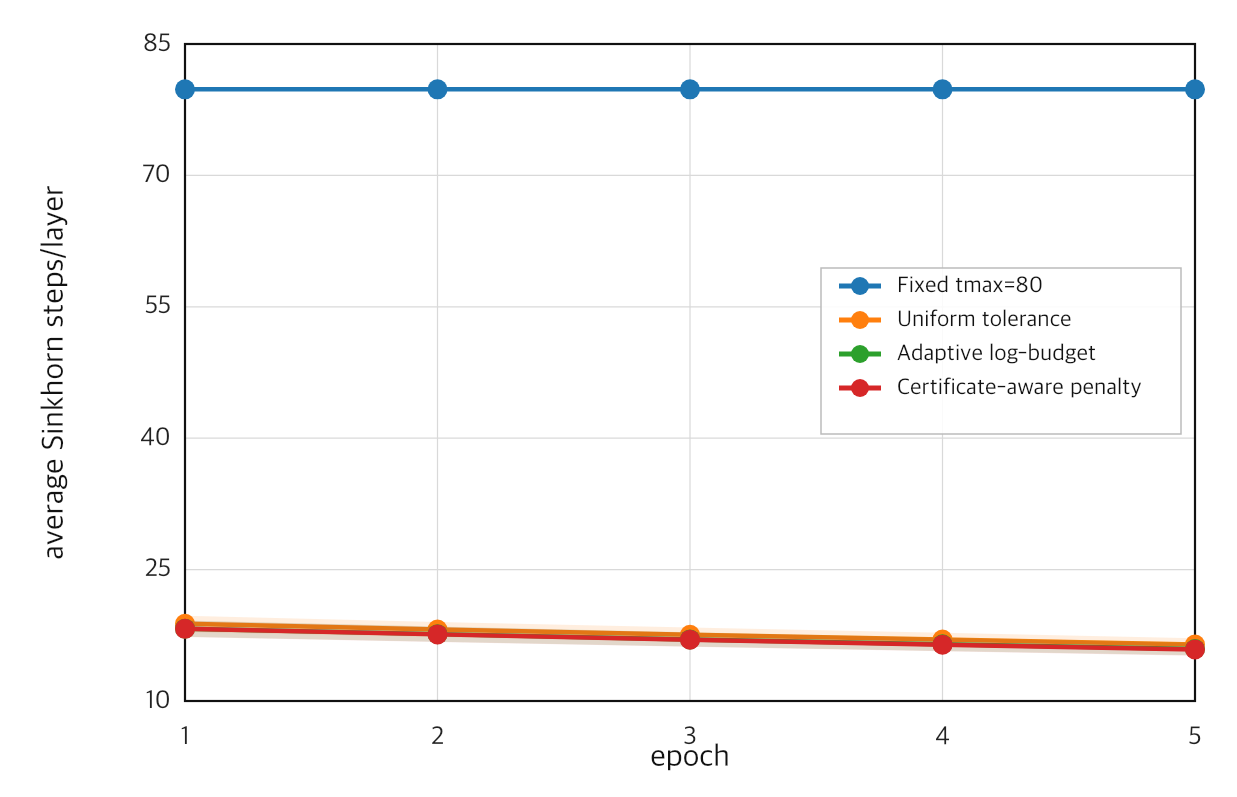
\includegraphics[width=\linewidth]{focused_avg_steps.png}
\caption{Average Sinkhorn steps.}
\end{subfigure}
\hfill
\begin{subfigure}{0.48\linewidth}
\centering
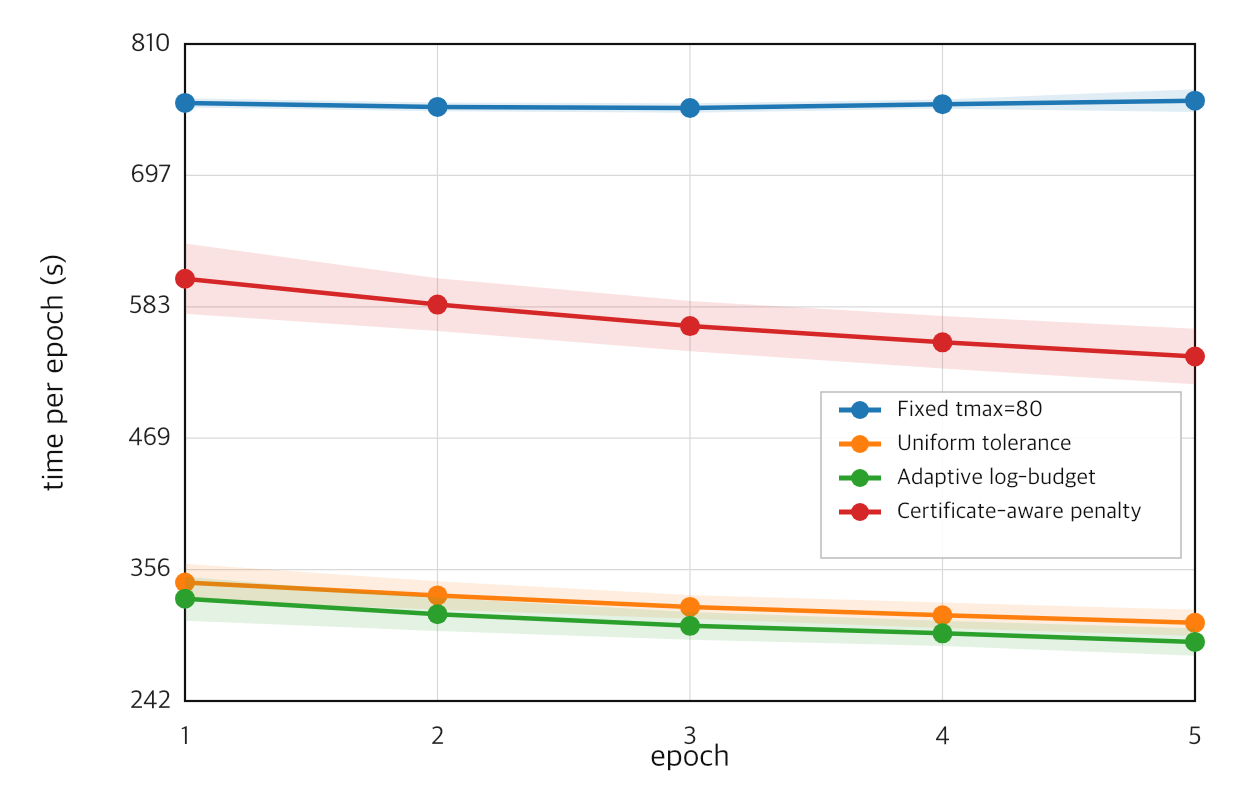
\includegraphics[width=\linewidth]{focused_time_per_epoch.png}
\caption{Time per epoch.}
\end{subfigure}

\medskip
\begin{subfigure}{0.48\linewidth}
\centering
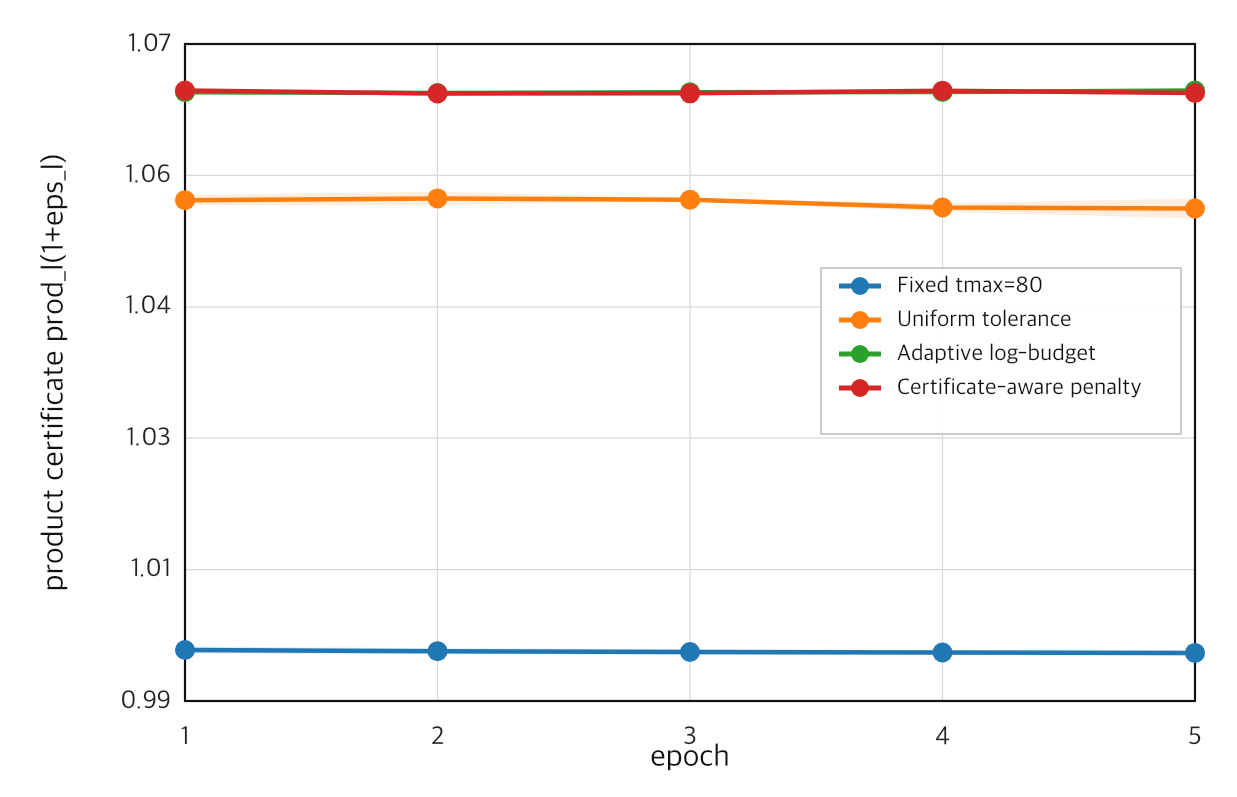
\includegraphics[width=\linewidth]{focused_product_cert.png}
\caption{Product certificate.}
\end{subfigure}
\hfill
\begin{subfigure}{0.48\linewidth}
\centering
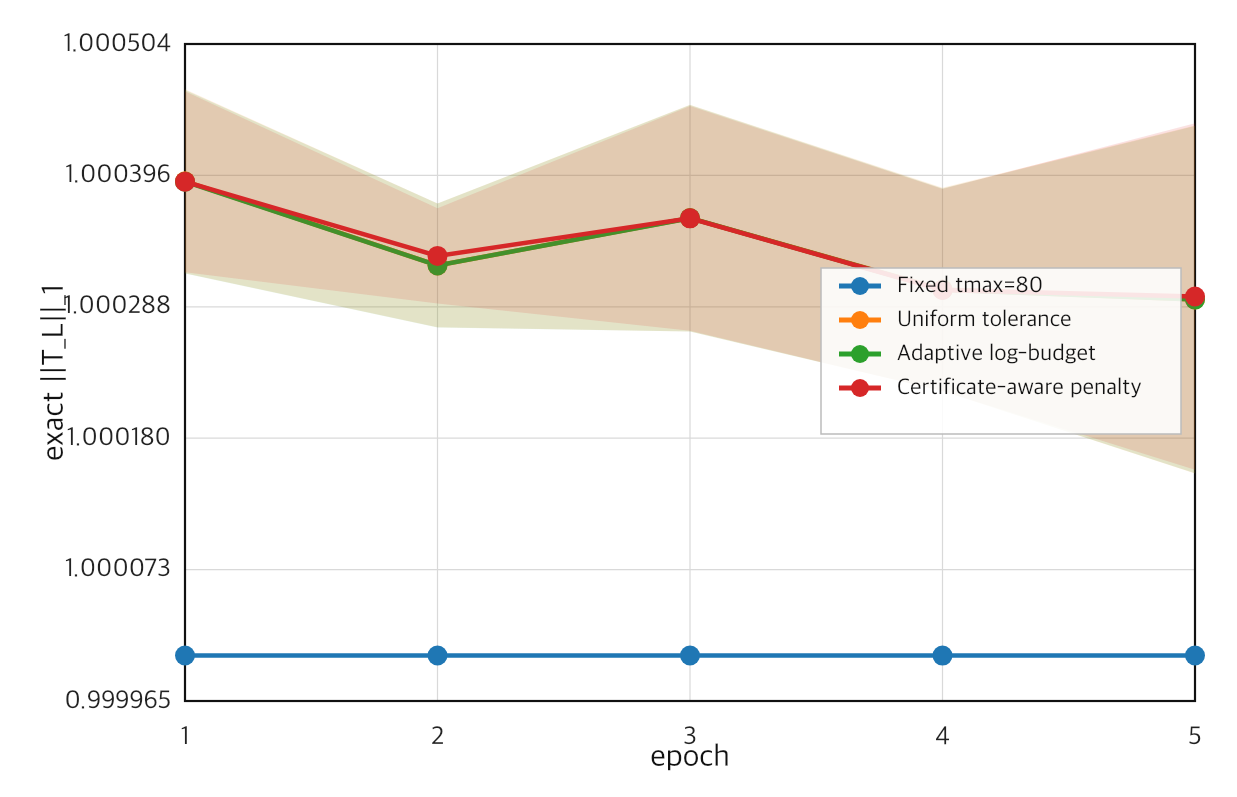
\includegraphics[width=\linewidth]{focused_exact_T1.png}
\caption{Exact propagated gain.}
\end{subfigure}
\caption{Focused controller-ablation trajectories over five epochs. Curves and
standard-deviation bands are computed only over seeds \(0,1,2\).}
\label{fig:focused_controller_curves}
\end{figure}

\paragraph{Temperature--clipping grid.}
Table~\ref{tab:temperature_clipping_grid} and Figure~\ref{fig:temperature_clipping_grid}
test the design inequality \eqref{eq:beta-R-cert} on random clipped logit matrices with
\(n=8\). The measured column errors are always below the finite-precision certificate
when the certificate is above the numerical floor. The grid also shows why the
temperature--clipping rule should be read as a conservative design certificate rather
than a sharp predictor: for large \(\beta R\), the worst-case certificate is nearly
vacuous even though the measured errors decrease rapidly with \(t_{\max}\).
\IfFileExists{paper-extra-experiments/logs/temperature_clipping_grid_table.tex}{%
\begin{table}[t]
\centering
\scriptsize
\begin{tabular}{ccccc}
\toprule
$\beta R$ & $t_{\max}$ & max measured $\varepsilon_c$ & certificate & max/cert. \\
\midrule
$0.5$ & $5$ & $9.79e-09$ & $8.41e-04$ & $1.16e-05$ \\
$0.5$ & $10$ & $6.66e-16$ & $3.74e-07$ & $1.78e-09$ \\
$0.5$ & $20$ & $2.22e-16$ & $7.36e-14$ & $0.00302$ \\
$0.5$ & $40$ & $2.22e-16$ & $<10^{-15}$ & --- \\
$0.5$ & $80$ & $2.22e-16$ & $<10^{-15}$ & --- \\
$1.0$ & $5$ & $3.81e-05$ & $0.161$ & $2.37e-04$ \\
$1.0$ & $10$ & $5.82e-10$ & $0.00995$ & $5.85e-08$ \\
$1.0$ & $20$ & $4.44e-16$ & $4.27e-05$ & $1.04e-11$ \\
$1.0$ & $40$ & $2.22e-16$ & $7.93e-10$ & $2.80e-07$ \\
$1.0$ & $80$ & $2.22e-16$ & $<10^{-15}$ & --- \\
$2.0$ & $5$ & $0.00563$ & $4.74$ & $0.00119$ \\
$2.0$ & $10$ & $6.38e-05$ & $3.1$ & $2.06e-05$ \\
$2.0$ & $20$ & $4.18e-10$ & $1.17$ & $3.57e-10$ \\
$2.0$ & $40$ & $2.22e-16$ & $0.21$ & $1.06e-15$ \\
$2.0$ & $80$ & $2.22e-16$ & $0.0104$ & $2.14e-14$ \\
$4.0$ & $5$ & $0.0763$ & $6.98$ & $0.0109$ \\
$4.0$ & $10$ & $0.0176$ & $6.98$ & $0.00252$ \\
$4.0$ & $20$ & $0.00147$ & $6.98$ & $2.11e-04$ \\
$4.0$ & $40$ & $6.28e-05$ & $6.97$ & $9.01e-06$ \\
$4.0$ & $80$ & $3.16e-10$ & $6.96$ & $4.54e-11$ \\
\bottomrule
\end{tabular}
\caption{Temperature--clipping grid for the design rule $\Psi_n(2\beta R\tanh(\beta R)^{2t_{\max}-1})$. Measured errors are maxima over 64 random clipped logit matrices with $n=8$. Entries shown as $<10^{-15}$ are below the numerical floor of this double-precision diagnostic.}
\label{tab:temperature_clipping_grid}
\end{table}

}{}

\begin{figure}[tbp]
\centering
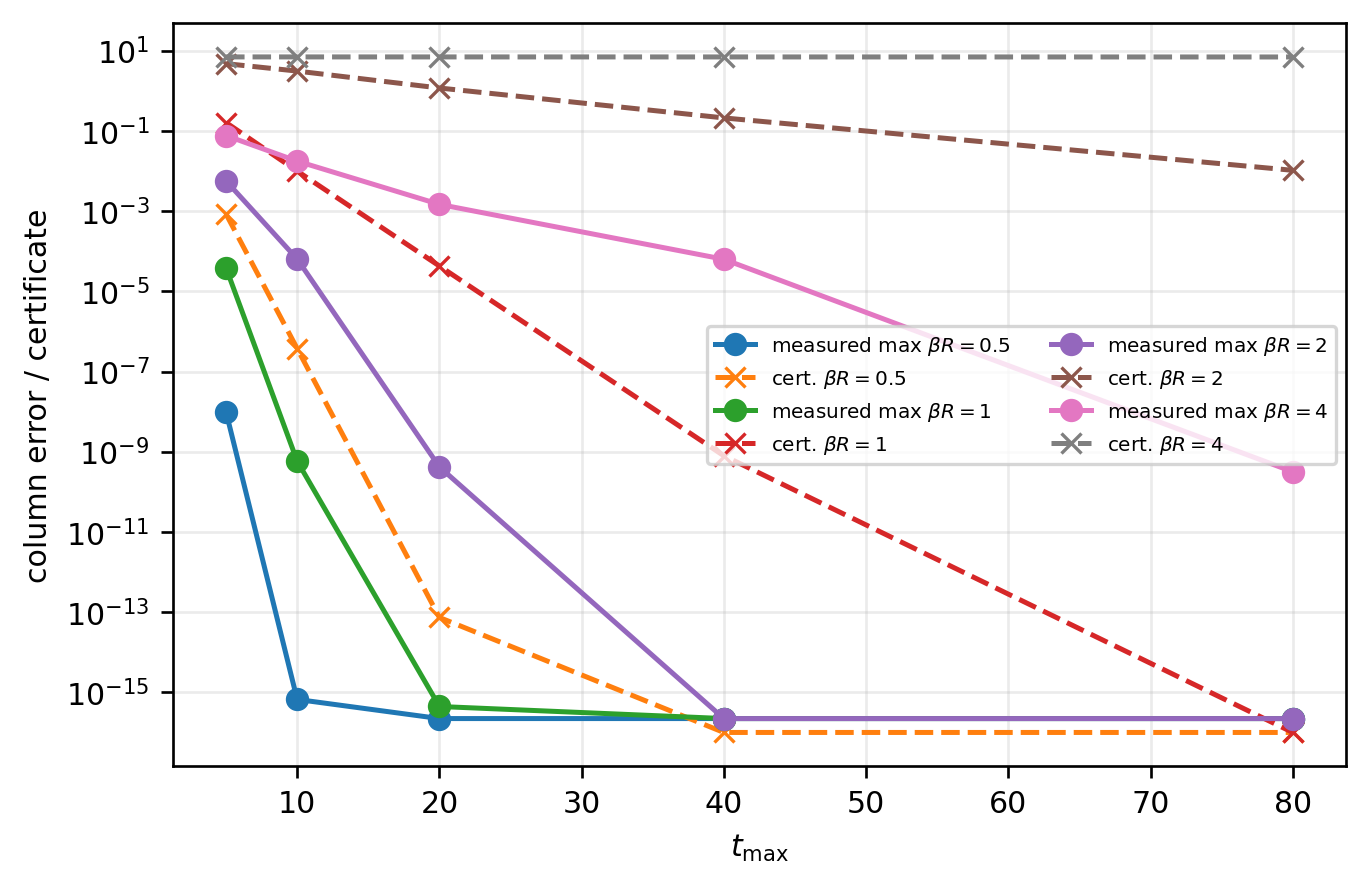
\includegraphics[width=0.72\linewidth]{temperature_clipping_grid.png}
\caption{Temperature--clipping diagnostic for the conservative design rule
\eqref{eq:beta-R-cert}. Solid curves are measured maximum column errors over random
clipped logits; dashed curves are the corresponding worst-case certificates.}
\label{fig:temperature_clipping_grid}
\end{figure}

\paragraph{Local-predictor curve.}
For trained adaptive Sinkhorn matrices, the extra runner records the full curve
\(\varepsilon_c^{(2t)}\) for \(t=1,\ldots,80\) and compares it with the \(\kappa\)-only
bound, the matrix-adaptive Hilbert bound, and the first- and second-order predictors from
Subsection~\ref{subsec:local-spectral}. Across the six recorded layer/seed curves, the
median absolute log\(_{10}\) error is \(0.26\) for the first-order predictor and \(0.19\)
for the second-order predictor, while the two global Hilbert certificates are more than
five orders of magnitude conservative at the median. Figure~\ref{fig:local_predictor_curve}
shows a representative trained layer.

\begin{figure}[tbp]
\centering
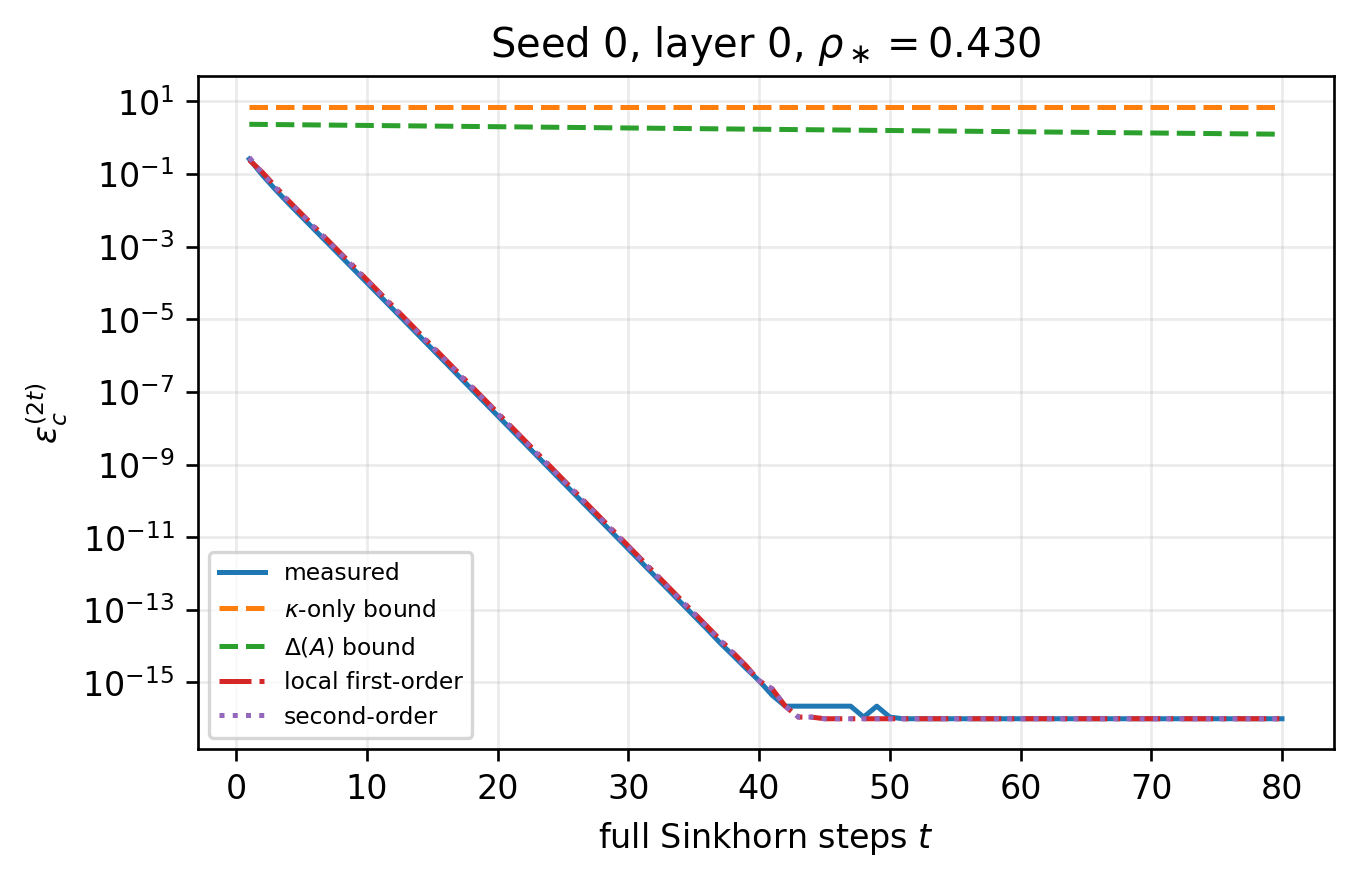
\includegraphics[width=0.72\linewidth]{local_predictor_seed0_layer0.png}
\caption{Representative local-predictor comparison on a trained adaptive Sinkhorn layer.
The local first- and second-order predictors track the measured Sinkhorn decay closely,
while the safe Hilbert certificates remain conservative.}
\label{fig:local_predictor_curve}
\end{figure}

\paragraph{Observed dynamic range.}
The final available median observed dynamic range across the Sinkhorn policies in the
focused run is \(\kappa_{\mathrm{obs}}\approx 1.27\times 10^4\). This does not contradict
the small-\(\kappa\) lookup table in Appendix~\ref{app:constants}: the table is an
illustrative conservative design example, whereas \(\kappa_{\mathrm{obs}}\) is a realized
diagnostic of trained clipped logits. Large observed dynamic range mainly explains why
the \(\kappa\)-only Hilbert bound is conservative, and why the numerical section reports
measured marginal errors, product certificates, exact propagated gains, and local
predictors next to the design rule.
\FloatBarrier

\paragraph{Generated figures.}
The real training log also supports the paper figures below. The plotted quantities are
epoch summaries across the GPU seeds rather than synthetic or random-matrix diagnostics;
the script \texttt{make\_paper\_plots.py} regenerates them directly from
\texttt{epoch\_logs.csv}. Auxiliary plots for test accuracy and the empirical final-step
ratio are written as checks, but the paper uses only the controller diagnostics shown here.

\begin{figure}[tbp]
\centering
\begin{subfigure}[tbp]{0.49\linewidth}
\centering
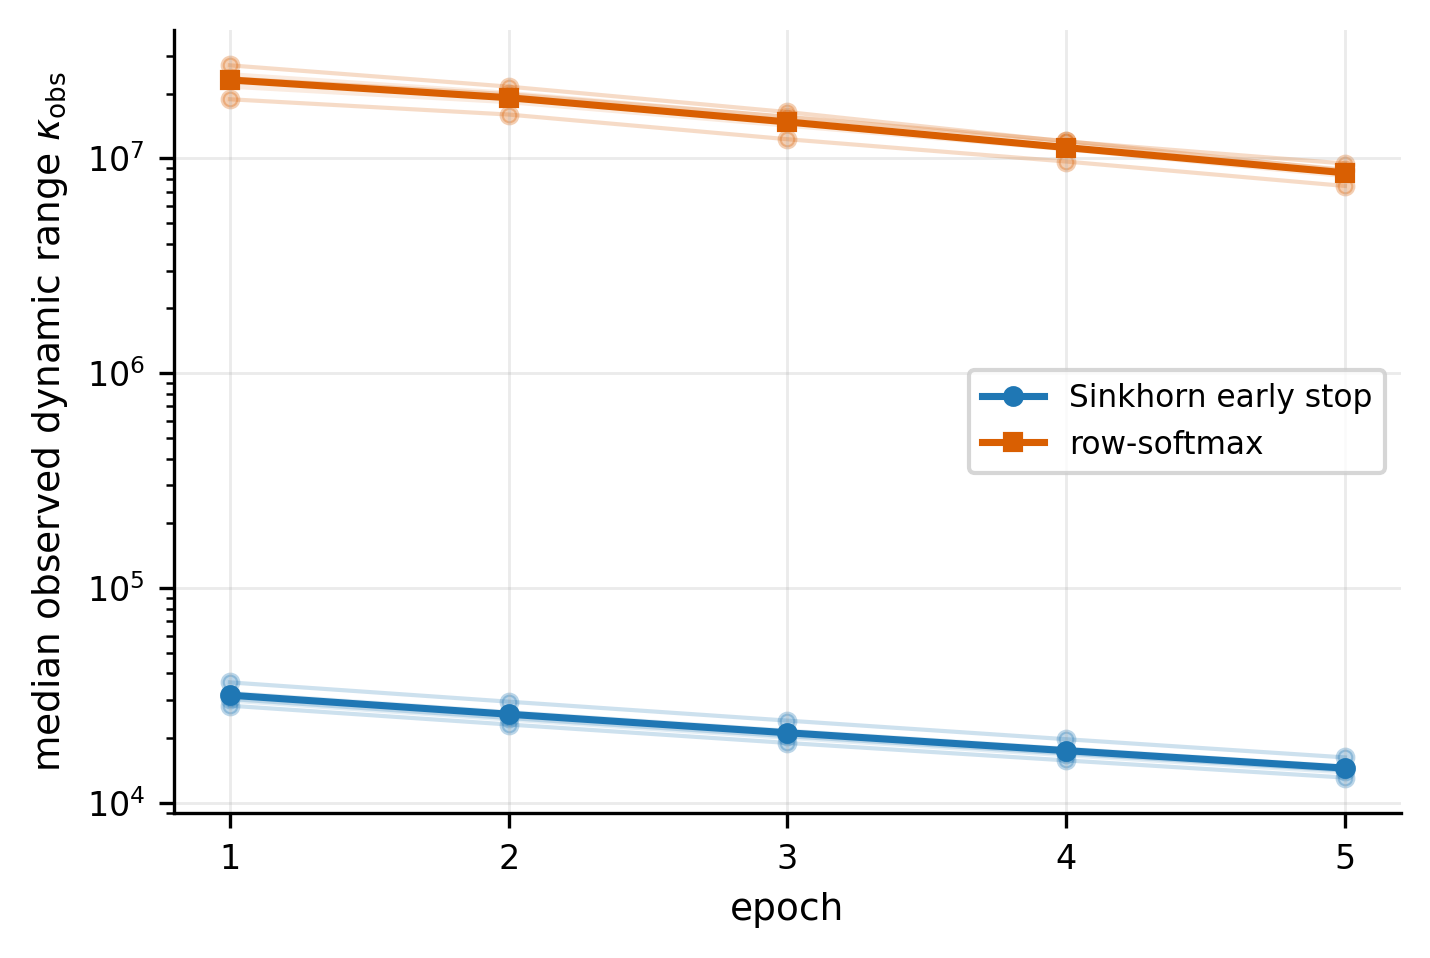
\includegraphics[width=\linewidth]{kappa_obs_log.png}
\caption{Observed dynamic range, log scale.}
\label{fig:kappa_obs}
\end{subfigure}\hfill
\begin{subfigure}[tbp]{0.49\linewidth}
\centering
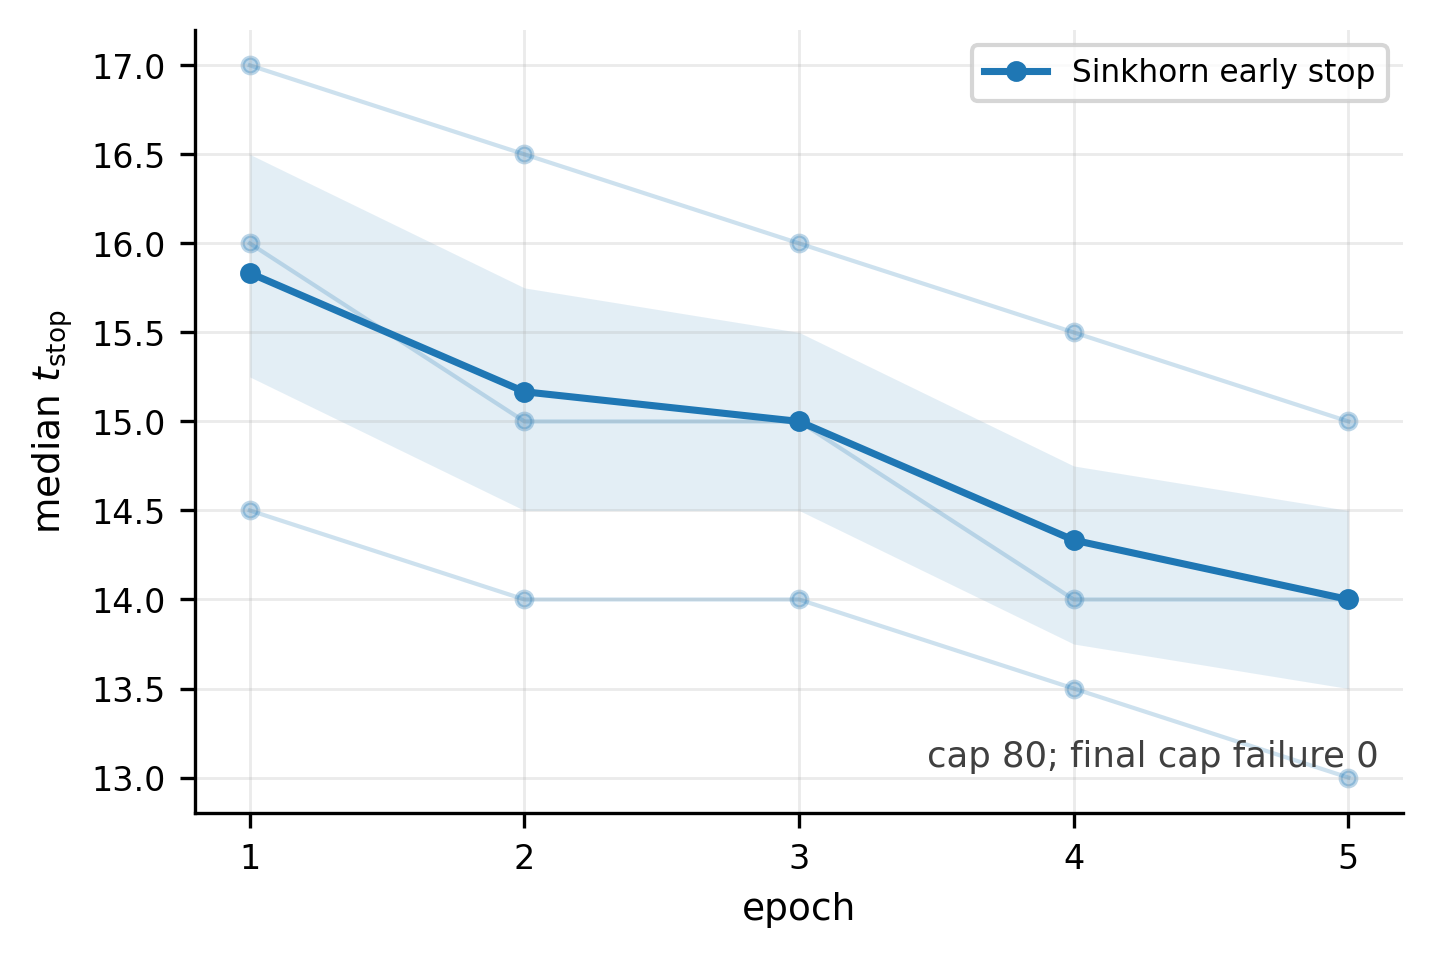
\includegraphics[width=\linewidth]{tstop_hist_early.png}
\caption{Early-stop step counts.}
\label{fig:tstop_hist}
\end{subfigure}
\caption{CIFAR-10 stress diagnostics for the finite-step Sinkhorn controller.}
\label{fig:kappa_tstop}
\end{figure}

\begin{figure}[tbp]
\centering
\begin{subfigure}[tbp]{0.49\linewidth}
\centering
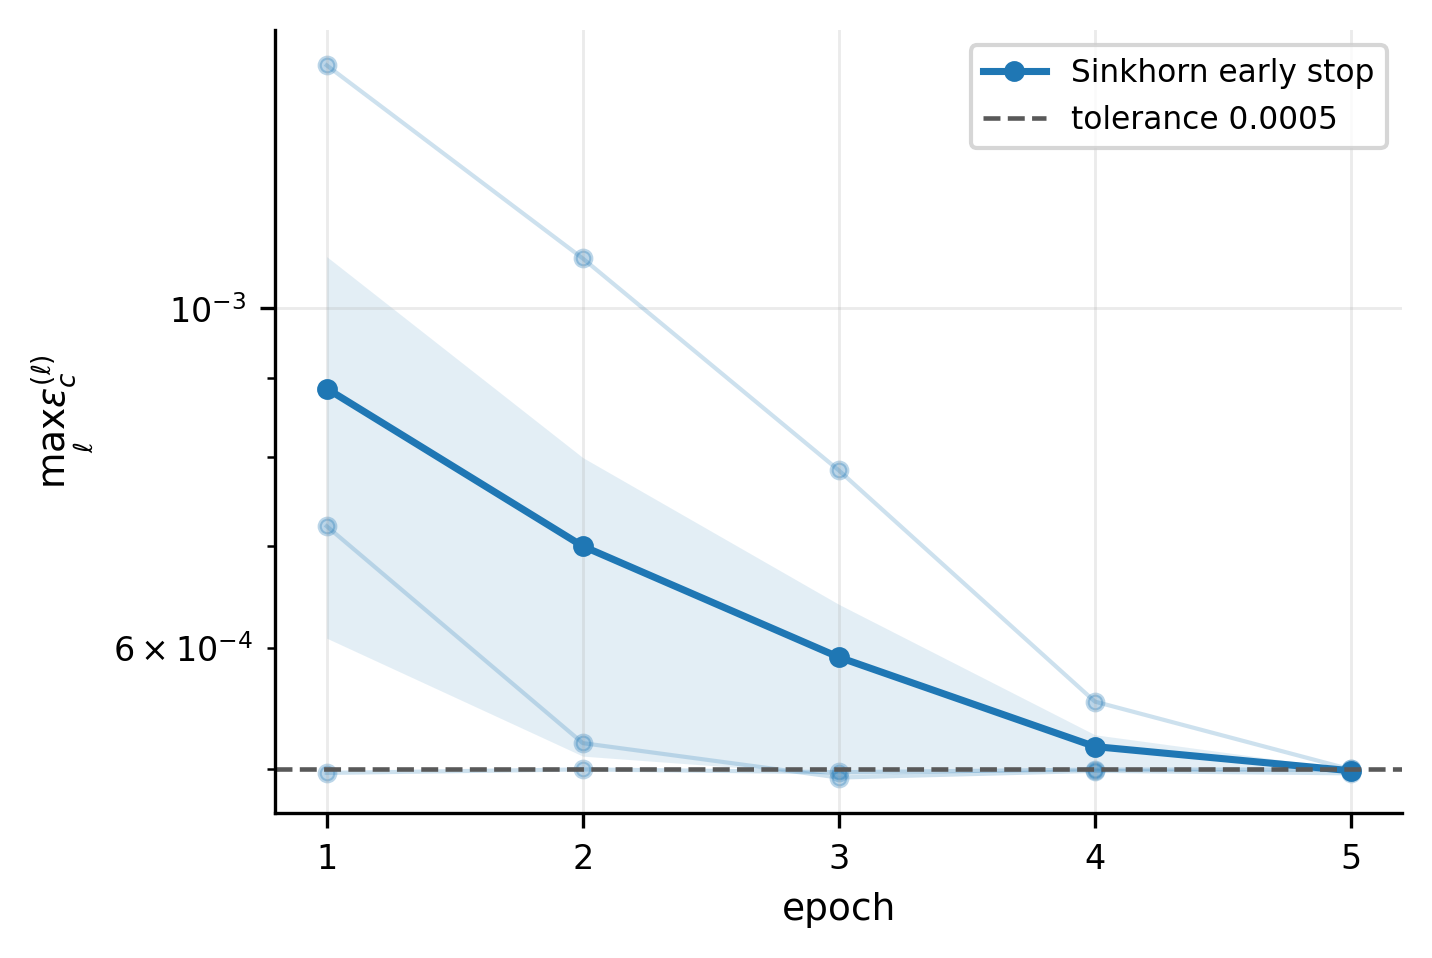
\includegraphics[width=\linewidth]{max_eps_c.png}
\caption{Maximum column-marginal error across layers.}
\end{subfigure}\hfill
\begin{subfigure}[tbp]{0.49\linewidth}
\centering
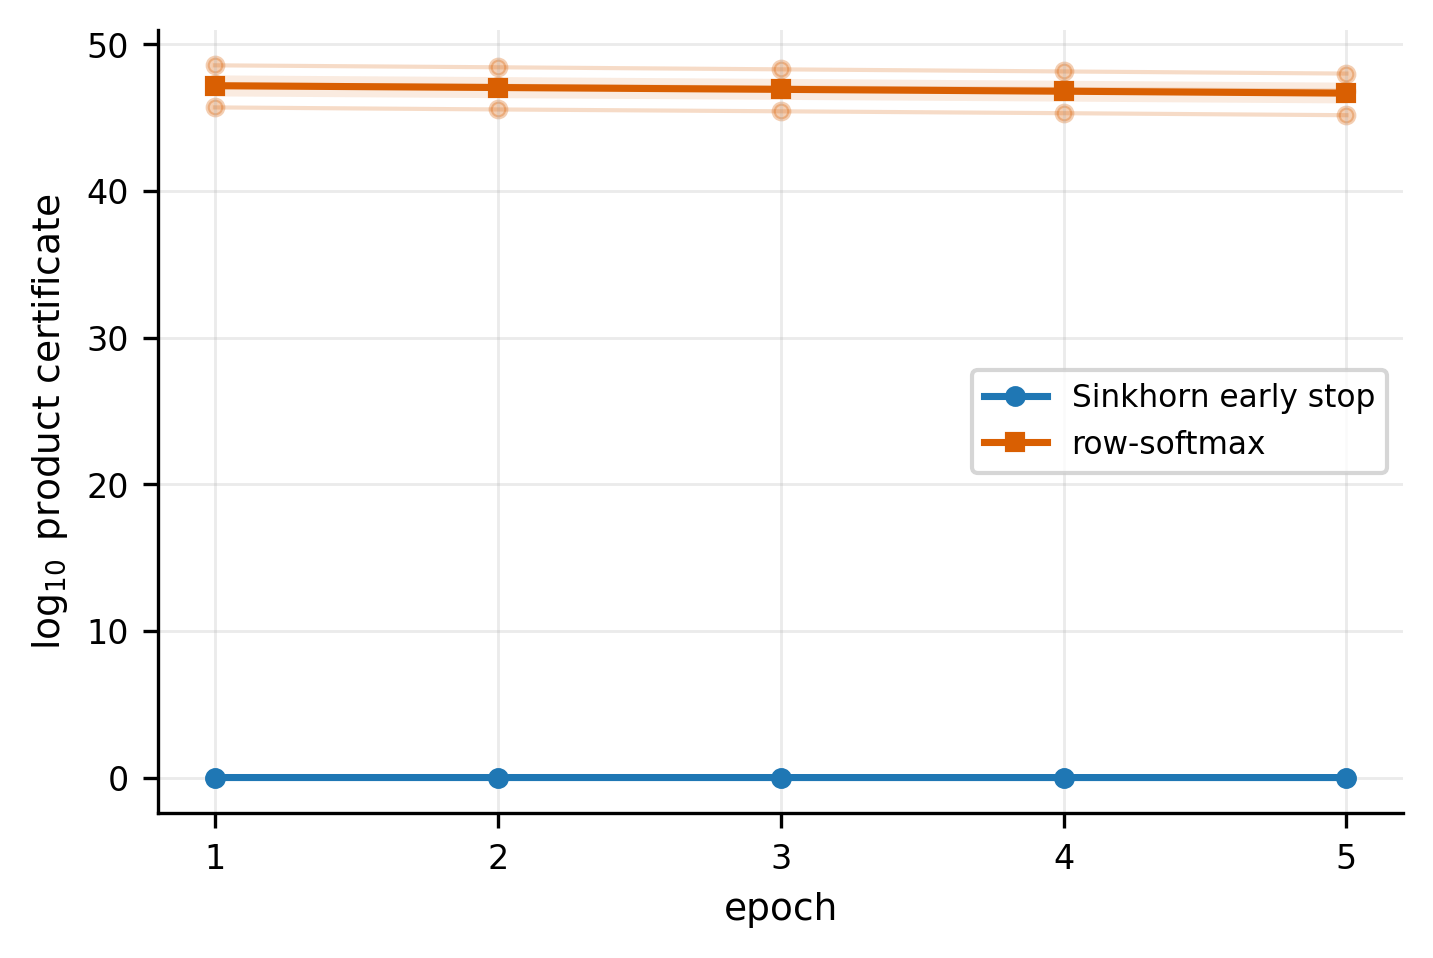
\includegraphics[width=\linewidth]{cert_bound.png}
\caption{Log-scale product certificate \(\prod_\ell(1+\varepsilon_c^{(\ell)})\).}
\end{subfigure}
\caption{Measured marginal error and the corresponding product certificate.}
\label{fig:cifar10_cert}
\end{figure}

\begin{figure}[tbp]
\centering
\begin{subfigure}[tbp]{0.49\linewidth}
\centering
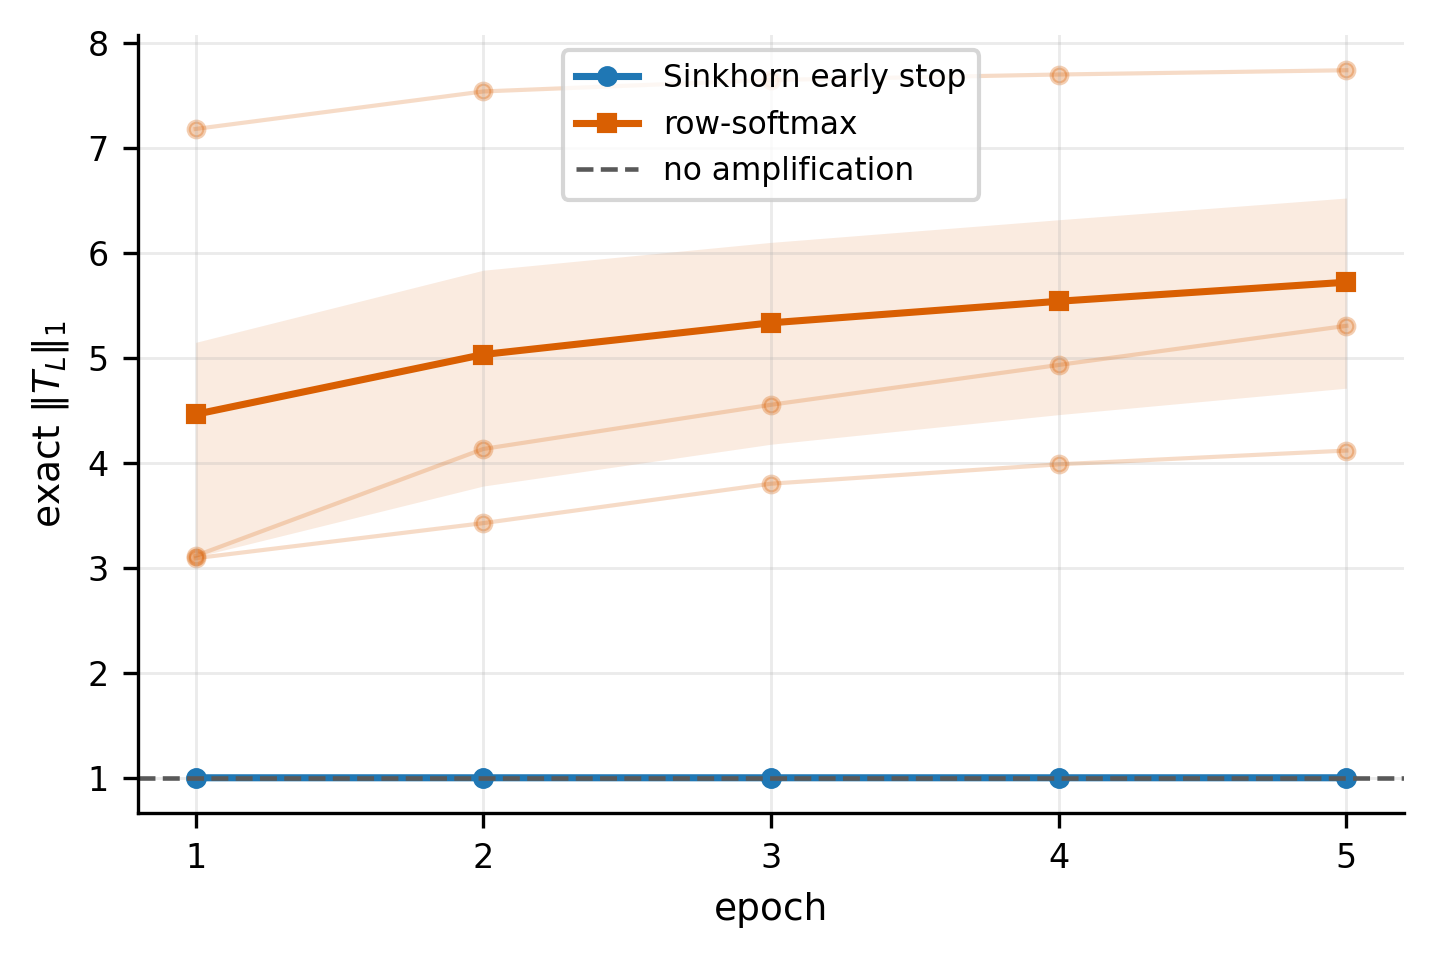
\includegraphics[width=\linewidth]{exact_T1.png}
\caption{Exact backward gain by vector propagation.}
\end{subfigure}\hfill
\begin{subfigure}[tbp]{0.49\linewidth}
\centering
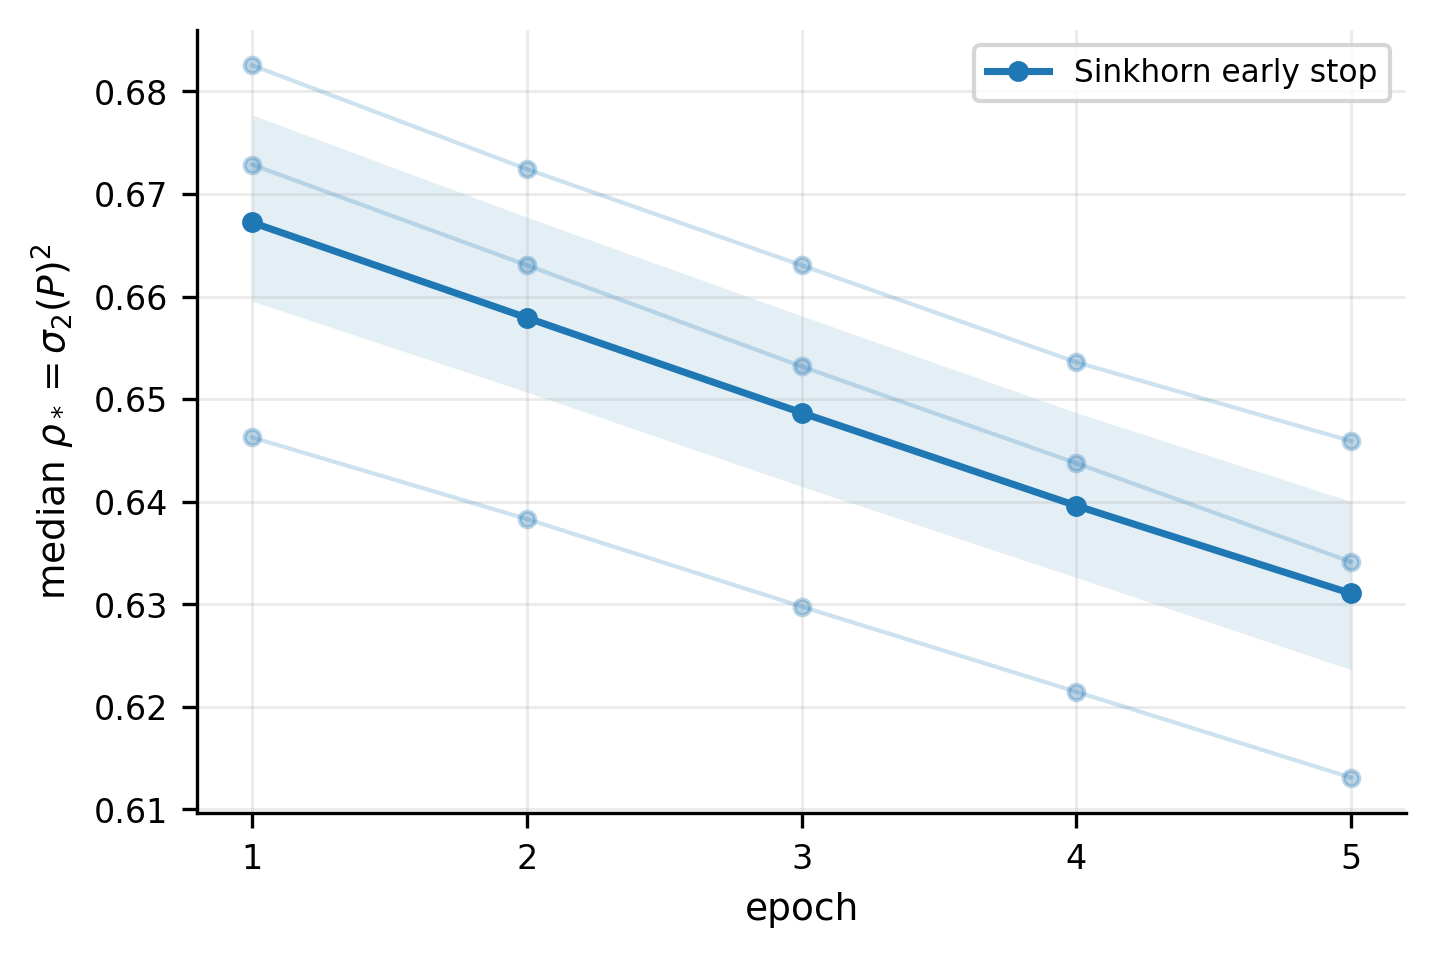
\includegraphics[width=\linewidth]{rho_star_median.png}
\caption{Median local spectral rate \(\rho_*\).}
\end{subfigure}
\caption{Exact realized gain and the local spectral predictor recorded during training.}
\label{fig:cifar10_gain_rho}
\end{figure}
\FloatBarrier

\paragraph{Scope of the reported experiments.}
The current code validates the fixed finite-step and early-stop controller diagnostics and
reports targeted diagnostics for adaptive global-budget stopping, the certificate-aware
penalty, the temperature--clipping rule, and the local spectral predictors. It does not
report a broad dataset or architecture benchmark; those larger comparisons are left out
rather than reported as unsupported numerical values.

\section{Discussion and practical guidance}\label{sec:discussion}
\subsection{Practical guidance}\label{subsec:guidance}
We summarize practical guidance for designing finite-step Sinkhorn mixers when the objective is to control \Amax
amplification across depth:
\begin{itemize}[leftmargin=*, itemsep=0.25em]
\item \textbf{Nonnegativity is required for worst-case \Amax certificates.}
The signed counterexample from Section~\ref{par:necessity} shows that marginal constraints alone cannot prevent arbitrarily large
$\|\cdot\|_\infty$, $\|\cdot\|_1$, or $\|\cdot\|_2$ amplification when signs are allowed.

\item \textbf{Depth-$L$ budgets translate into per-layer tolerances.}
For small errors, a composite budget $\|T_L\|_1\le B_1$ corresponds to
$\sum_{\ell=1}^L \varepsilon_c^{(\ell)}\lesssim \log B_1$, and a simple uniform choice is
$\varepsilon_c \approx \log(B_1)/L$ (see Remark~\ref{rem:depth_sensitivity}).

\item \textbf{Given a target tolerance, $(\kappa,t_{\max})$ can be selected via the finite-step rule.}
Given a target $\varepsilon_c$, the corrected finite-step rule (Theorem~\ref{thm:sinkhorn}) provides a sufficient $t_{\max}$ through
$\Psi_n\!\left((\log\kappa)q^{2t_{\max}-1}\right)\le\varepsilon_c$. Smaller $\kappa$ improves contraction (fewer steps) but restricts routing selectivity (see Remark~\ref{rem:tradeoff}).

\item \textbf{For prediction, use the local spectral rate.}
The $\kappa$-only bound is a worst-case certificate. When a numerical prediction of the marginal-error curve is needed, compute the Sinkhorn limit $P$ and use the local rate $\sigma_2(P)^2$ and predictor \eqref{eq:local-spectral-predicted-error}.

\item \textbf{For training, use a global-budget controller rather than a fixed tolerance whenever possible.}
The adaptive rule in Lemma~\ref{lem:adaptive-budget} spends the remaining log-budget across the remaining layers, and the exact vector propagation certificate in Remark~\ref{rem:exact-backward-gain} measures the realized gain.

\item \textbf{For implementation, calibrate temperature and clipping jointly.}
Corollary~\ref{cor:temperature-clipping} converts $(\beta,R,t_{\max})$ directly into a conservative tolerance. Large $\beta R$ increases selectivity but slows the worst-case Sinkhorn certificate.
\end{itemize}

\begin{remark}[Transfer beyond mHC: attention and message passing] 
The results in Sections~\ref{sec:amax}--\ref{sec:sinkhorn} apply verbatim to any architecture whose depth-wise propagation includes
a product of \emph{entrywise nonnegative} approximately bistochastic mixing matrices. This includes, for example,
(i) Sinkhorn-normalized attention maps (e.g.,\ doubly-stochastic attention) when the normalization is performed on the relevant
(unmasked) support, and (ii) reweighted graph message-passing operators that are constrained to be approximately doubly stochastic.
These guarantees assume strict positivity on the support being normalized; masked attention or sparse normalization can violate
the standing assumptions of Section~\ref{sec:sinkhorn} and requires separate treatment (e.g., restricting to the unmasked block).

In these settings, Theorem~\ref{prop:product} certifies worst-case amplification of the \emph{mixing sub-operator}.
Full-block stability still requires coupling this certificate with bounds on the remaining components
(e.g., projections/MLPs/normalization), as recorded in Appendix~\ref{app:jacobian}.
\end{remark}


\subsection{Limitations}\label{subsec:limitations}
Our results provide \emph{sufficient} stability certificates tailored to the \Amax diagnostic and the finite-step Sinkhorn
mechanism studied here. The analysis is intentionally modular, and several aspects are outside the present scope.

\noindent\textbf{Worst-case nature and conservatism.}
Our deterministic certificates are worst-case and can be conservative. The product bound in Theorem~\ref{prop:product} may be loose when mixers have additional structure, although the realized backward gain can be computed exactly by Remark~\ref{rem:exact-backward-gain}. Similarly, the Hilbert-metric constants in Theorem~\ref{thm:sinkhorn} are safe global certificates. The local envelope in Proposition~\ref{thm:local-envelope} is much sharper for matrices whose logarithmic Sinkhorn orbit lies near the limit, but it is still local. The first- and second-order predictors explain typical numerical behavior; they are not uniform worst-case guarantees.

\noindent\textbf{Finite-step Sinkhorn constants.}
The step-count rule uses Hilbert-metric contraction bounds. The matrix-adaptive diameter $\Delta(A)$ and initialization $\delta_0$ already improve the $\kappa$-only estimate, but they remain global certificates. The derivative envelope based on $\rho_R$ and $\lambda_R$ is sharper and non-asymptotic on a verified local ball. The first-order rate $\sigma_2(P)^2$ gives the late-stage slope, while the second-order expansion improves the first few finite steps.

\noindent\textbf{Nonlinear blocks and full-network training dynamics.}
The influence of the nonlinear block $F$ enters only through Jacobian norm bounds such as Proposition~\ref{thm:full-jac} and Corollary~\ref{cor:jacobian-cert}.
We do not model how training shapes $\widetilde{\Hres}^{(\ell)}$ (and hence $\kappa$ or marginal errors), nor do we analyze how
the certificates interact with optimization, data distribution, or generalization.

\noindent\textbf{Architectural and implementation choices.}
Our statements track the streams-as-rows convention and a specific normalization order for finite-step Sinkhorn. Other conventions
(e.g.\ streams-as-columns) or implementation details (e.g.\ damping, mixed precision, sparse mixers) require straightforward but
explicit translation, and can affect which marginal error is nontrivial at the output.

Connecting worst-case certificates to learned behavior would require sharper finite-step constants or additional structure beyond marginal errors.

\subsection{Future work}\label{subsec:future_work}
Three directions would improve practicality: (i) turning the local derivative envelope into cheap certified code for each batch/layer, including reliable upper bounds for $\rho_R$ and $\lambda_R$; (ii) expanding the controller and certificate-penalty ablations across datasets and architectures, including more efficient implementations of the differentiable penalty; and (iii) deriving tighter full-network bounds that couple mixer certificates to the Jacobians of the nonlinear blocks, rather than using a uniform $L_F$ surrogate.





\section{Conclusion}\label{sec:conclusion}

We developed deterministic finite-step certificates for nonnegative
Sinkhorn-normalized stream mixers.  The central point is that, for nonnegative
matrices, marginal errors are not merely normalization diagnostics: they are
induced-norm certificates.  In the \texttt{column-then-row} Sinkhorn order, the
output row sums are exact in ideal arithmetic and the remaining output column
defect gives a backward \Amax budget for the depth-wise mixer product.  Hilbert
projective contraction turns logit dynamic range and finite Sinkhorn step count
into a conservative design-time tolerance, while matrix-specific local analysis
explains why realized convergence is often much faster than the worst-case
bound.

The resulting theory supports adaptive early stopping, budget tracking, and
exact realized gain diagnostics for the mixing pathway.  The focused ablations
show that, at the same depth-wise product budget, adaptive log-budget stopping
matches the uniform tolerance rule in accuracy and exact backward gain while
using modestly fewer Sinkhorn steps.  The certificate-aware penalty preserves
the same stability diagnostics but is slower in the current implementation, so
it should be read as a feasibility/control diagnostic rather than as a speedup.
Extending these mixer-path certificates to full network-level guarantees
requires additional control of the nonlinear residual branches, and extending
the finite-step theory to masked or sparse supports remains an important
direction for future work.


 \section*{Reproducibility Statement}
We provide scripts to regenerate all figures and tables, with fixed random seeds and commands referenced by figure/table number. Because numerical behavior depends on implementation details, we report the Sinkhorn dtype, the positivity floor $\epsfloor$, clipping/temperature settings, and the early-stopping tolerance; these quantities directly affect measured marginal errors and the resulting certificates.

 


\medskip
\noindent\textbf{Code:} The code, raw CSV/JSON logs, regeneration scripts,
fixed seeds, and a CPU smoke test are available at
\begin{center}
\small\url{https://github.com/MaKosmakov/finite-step-sinkhorn-certificates}
\end{center}

\noindent\textbf{Data:} The Kaggle runs use the
\href{https://www.kaggle.com/datasets/pankrzysiu/cifar10-python}{CIFAR-10 Python dataset},
mounted at
\begin{center}
\small\texttt{/kaggle/input/cifar10-python}
\end{center}
\noindent Local runs may instead point \texttt{--data\_root} to any standard
CIFAR-10 Python archive or extracted CIFAR-10 root.
 

\medskip
\noindent\textbf{Exact regeneration commands.}
\begin{lstlisting}[language=sh]
# CPU smoke test on real CIFAR-10 data; validates code paths only.
MPLCONFIGDIR=/tmp/mplconfig python train_cifar10_mhc.py \
  --profile baseline --epochs 1 --seeds 0 \
  --num_workers 0 --batch_size 64 \
  --n_streams 4 --d 32 --depth 4 \
  --sinkhorn_t_max 8 --sinkhorn_eps_tol 5e-4 \
  --max_train_batches 1 --max_eval_batches 1 \
  --data_root /kaggle/input/cifar10-python \
  --out_dir results-cpu-smoke

# Full CIFAR-10 stress run used for paper diagnostics.
python train_cifar10_mhc.py \
  --profile stress_full --epochs 5 --seeds 0 1 2 \
  --batch_size 256 --num_workers 4 \
  --data_root /kaggle/input/cifar10-python \
  --out_dir results-stressed-cap80 \
  --amp

# Extra diagnostics: temperature-clipping grid and local-predictor curves.
python paper_extra_experiments_kaggle.py

# Focused controller ablation used for Table 5 and Figure 2.
python paper_extra_experiments_3seeds_5epochs_kaggle.py
python paper-extra-experiments/regenerate_focused_ablation_3seed.py \
  paper-extra-experiments-3seeds-5epochs/logs/focused_ablation_epoch_logs.csv \
  paper-extra-experiments
\end{lstlisting}

\noindent The repository command manifest gives the full, paper-indexed list
of commands and environment details.


\appendix


\section{Implementation pseudocode for certificate bookkeeping}\label{app:implementation-pseudocode}

The following listings are not separate algorithmic contributions.  They specify
the bookkeeping used to evaluate the finite-step certificates in implementation.

\begin{lstlisting}[language=Python,caption={Early stopping for \texttt{column-then-row} Sinkhorn to a column-marginal tolerance.},label={lst:sinkhorn_earlystop}]
def sinkhorn_col_row(M, t_max, eps_tol, floor=1e-12):
    # M: positive matrix (e.g., exp(beta * logits))
    X = np.maximum(M.copy(), floor)
    tiny = np.finfo(X.dtype).tiny

    for t in range(1, t_max + 1):
        # Full step: column then row normalization
        X /= np.maximum(X.sum(axis=0, keepdims=True), tiny)  # columns
        X /= np.maximum(X.sum(axis=1, keepdims=True), tiny)  # rows

        # column-marginal error at full-step output S^{(2t)}
        eps_c = np.max(np.abs(X.sum(axis=0) - 1.0))
        if eps_c <= eps_tol:
            return X, t  # t is the number of full steps used

    return X, t_max
\end{lstlisting}

\begin{lstlisting}[language=Python,caption={Adaptive global-budget finite-step Sinkhorn early stopping.},label={lst:adaptive_budget_sinkhorn}]
def sinkhorn_global_budget(logits_list, B1, t_cap, eps_floor=1e-12):
    """Return mixers and a realized product certificate."""
    L = len(logits_list)
    b = math.log(B1)
    s = 0.0
    H_list, eps_list, step_list = [], [], []
    budget_failed = False

    for ell, C in enumerate(logits_list):
        remaining_layers = L - ell
        eps_target = math.exp((b - s) / remaining_layers) - 1.0

        A = torch.exp(C).clamp_min(eps_floor)
        H, eps_c, steps = sinkhorn_until_column_tol(
            A, eps_target=eps_target, t_cap=t_cap, eps_floor=eps_floor
        )

        H_list.append(H)
        eps_list.append(eps_c)
        step_list.append(steps)

        if float(eps_c) > eps_target:
            budget_failed = True
        s += math.log1p(float(eps_c))

    product_certificate = math.exp(s)
    return H_list, eps_list, step_list, product_certificate, budget_failed
\end{lstlisting}

\section{Auxiliary proof details}\label{app:auxiliary-proofs}

\paragraph{Proof of Lemma~\ref{lem:Psi}.}
Let \(a:=\max_i u_i\), \(b:=\min_i u_i\), and \(r:=a/b=e^\delta\ge1\).
The mean constraint gives \(b\le1\le a\). For the upper deviation, fixing the
ratio \(a/b=r\) and the mean, the largest possible value of \(a\) occurs when
one entry is \(a\) and the remaining \(n-1\) entries are \(b\). Hence
\[
        a\le \frac{nr}{r+n-1},
        \qquad
        a-1\le \frac{(n-1)(r-1)}{r+n-1}.
\]
For the lower deviation, the smallest possible value of \(b\) occurs when one
entry is \(b\) and the remaining \(n-1\) entries are \(a\). Thus
\[
        b\ge \frac{n}{1+(n-1)r},
        \qquad
        1-b\le \frac{(n-1)(r-1)}{1+(n-1)r}.
\]
Since \(1+(n-1)r\ge r+n-1\) for \(n\ge2\) and \(r\ge1\), the lower-tail bound is
no larger than the upper-tail bound. Therefore
\[
        \|u-\ones\|_{\infty,\mathrm{vec}}
        \le
        \frac{(n-1)(r-1)}{r+n-1}
        =\Psi_n(\delta).
\]
Solving \(\Psi_n(\delta)\le\varepsilon\) for \(r=e^\delta\) gives
\eqref{eq:Psi-inv}.

\paragraph{Proof of Lemma~\ref{lem:Gamma}.}
Since \(z=\Pi\log u\) and \(n^{-1}\sum_i u_i=1\), there is a unique scalar
normalization such that
\[
        u_i=\frac{n e^{z_i}}{\sum_{k=1}^n e^{z_k}}.
\]
We first maximize a single coordinate. Under the constraints \(\sum_i z_i=0\)
and \(\|z\|_2\le\eta\), the largest possible value of one coordinate is
\[
        a=\sqrt{\frac{n-1}{n}}\,\eta,
\]
attained when the remaining coordinates all equal \(-a/(n-1)\). Indeed, if
\(z_i=a\) is fixed, the sum of the other coordinates is \(-a\); Jensen's
inequality gives
\[
        \sum_{k\ne i}e^{z_k}
        \ge
        (n-1)e^{-a/(n-1)},
\]
with equality exactly in the equal-tail configuration. Therefore
\[
        u_i
        \le
        \frac{n e^a}{e^a+(n-1)e^{-a/(n-1)}}.
\]
This gives the upper-tail deviation \(\Gamma_n(\eta)\).

It remains to check that the lower-tail deviation is not larger. Put
\[
        r:=\exp\!\left(\frac{n}{n-1}a\right)\ge1.
\]
For the upper-tail extremizer, the maximal coordinate is
\[
        U=\frac{nr}{r+n-1}.
\]
For the lower-tail extremizer, where one coordinate is \(-a\) and the other
\(n-1\) coordinates are \(a/(n-1)\), the minimal coordinate is
\[
        L=\frac{n}{1+(n-1)r}.
\]
The upper and lower deviations are \(U-1\) and \(1-L\). A direct calculation
gives
\begin{equation}\label{eq:Gamma-tail-comparison}
        (U-1)-(1-L)
        =U+L-2
        =
        \frac{(n-1)(n-2)(r-1)^2}{(r+n-1)(1+(n-1)r)}
        \ge0.
\end{equation}
Thus the one-spike upper-tail value controls the full \(\ell_\infty\)
deviation. Expanding \eqref{eq:Gamma-def} at \(\eta=0\) gives
\eqref{eq:Gamma-small}.

\section{Second-order local predictor formulas}\label{app:second-order-predictor}

The second-order diagnostic predictor keeps the quadratic terms in the
logarithmic Sinkhorn map.  With \(K=PP^\top\), define
\begin{equation}\label{eq:QF-QL}
        Q_F(x)
        :=
        -P\big((P^\top x)^{\odot2}\big)
        +\frac12 K(x^{\odot2})
        +\frac12 (Kx)^{\odot2},
\end{equation}
\begin{equation}\label{eq:QL}
        Q_L(x)
        :=
        \frac12 P^\top(x^{\odot2})
        -\frac12 (P^\top x)^{\odot2}.
\end{equation}
Then
\begin{equation}\label{eq:F-L-second-expansion}
        \mathcal F(x)=Kx+\Pi Q_F(x)+O(\|x\|^3),
        \qquad
        \mathcal L(x)=\Pi P^\top x+\Pi Q_L(x)+O(\|x\|^3).
\end{equation}
Set
\begin{equation}\label{eq:second-order-x}
        x_t^{[1]}:=K^t x_0,
        \qquad
        x_t^{[2]}
        :=
        K^t x_0+
        \sum_{s=0}^{t-1}K^{t-1-s}\Pi Q_F(K^s x_0).
\end{equation}
The second-order centered log-column predictor is
\begin{equation}\label{eq:second-order-predictor-log}
        \ell_t^{[2]}
        :=
        \Pi\Big[
        P^\top x_t^{[2]}+Q_L(x_t^{[1]})
        -P^\top x_{t-1}^{[2]}-Q_L(x_{t-1}^{[1]})
        \Big].
\end{equation}
Finally define
\begin{equation}\label{eq:second-order-predictor-eps}
        \widehat v_t^{[2]}
        :=
        \frac{n\exp(\ell_t^{[2]})}{\sum_{j=1}^n\exp((\ell_t^{[2]})_j)},
        \qquad
        \widehat\varepsilon_{c,2}^{(2t)}
        :=
        \|\widehat v_t^{[2]}-\ones\|_{\infty,\mathrm{vec}}.
\end{equation}
For each fixed \(t\),
\begin{equation}\label{eq:second-order-accuracy}
        z_t=\ell_t^{[2]}+O_t(\|x_0\|^3).
\end{equation}
Thus \eqref{eq:second-order-predictor-eps} is the natural finite-step prediction
to compare with early numerical points, while
\eqref{eq:local-spectral-predicted-error} gives the asymptotic slope.


\section{One explicit sufficient instantiation of the finite-step rule}\label{app:constants}

This appendix provides an explicit instantiation of the corrected step-count rule in Theorem~\ref{thm:sinkhorn}.

Assume the positive pre-scaling matrix $S^{(0)}$ has dynamic range
\begin{equation}
\kappa:=\frac{\max_{i,j} S^{(0)}_{ij}}{\min_{i,j} S^{(0)}_{ij}}.
\end{equation}
By Birkhoff--Bushell contraction theory for positive maps in the Hilbert projective metric
\cite{Birkhoff1957,Bushell1973}, a conservative contraction bound is
\begin{equation}\label{eq:app-q}
q =\frac{\kappa-1}{\kappa+1}.
\end{equation}
The corrected output column-marginal estimate in the \texttt{column-then-row} order is
\begin{equation}\label{eq:app-corrected-design-law}
\varepsilon_c^{(2t)}
\le
\Psi_n\!\left((\log\kappa)q^{2t-1}\right),
\qquad t\ge1.
\end{equation}
Thus it suffices to choose $t_{\max}$ so that
\begin{equation}\label{eq:app-tmax-corrected}
t_{\max}
\ge
\frac12
\left[
1+
\frac{\log\!\left((\log\kappa)/\Psi_n^{-1}(\bar\varepsilon)\right)}
{\log(1/q)}
\right],
\end{equation}
rounded up.

\paragraph{Numerical examples for $n=4$.}
For target marginal error $\bar\varepsilon=10^{-3}$ and $n=4$, the table below reports
$q=(\kappa-1)/(\kappa+1)$, $\log\kappa$, and the sufficient $t_{\max}$ obtained from
Equation~\eqref{eq:app-tmax-corrected} with $\Psi_n^{-1}$ from Equation~\eqref{eq:Psi-inv}.

\begin{center}
\begin{tabular}{@{}cccc@{}}
\toprule
$\kappa$ & $q=(\kappa-1)/(\kappa+1)$ & $\log\kappa$ & sufficient $t_{\max}$\\
\midrule
2& 0.333 & 0.693 & 4\\
5& 0.667 & 1.609 & 10 \\
10 & 0.818 & 2.303 & 20 \\
\bottomrule
\end{tabular}
\end{center}

\begin{table}[tbp]
\centering
\small
\begin{tabular}{@{}l c@{}}
\toprule
quantity & value \\
\midrule
$n$ & $8$ \\
$\kappa$ & $10$ \\
$q=(\kappa-1)/(\kappa+1)$ & $0.818182$ \\
$\log\kappa$ & $2.30259$ \\
$\Psi_n^{-1}(10^{-3})$ & $0.00114237$ \\
sufficient $t_{\max}$ from \eqref{eq:app-tmax-corrected} & $20$ \\
$\Psi_n\!\big((\log\kappa)q^{2t_{\max}-1}\big)$ at $t_{\max}=20$ & $8.045\times 10^{-4}$ \\
\bottomrule
\end{tabular}
\caption{Numerical evaluation of the corrected explicit design-law bound (Theorem~\ref{thm:sinkhorn}) for $(n,\kappa,\bar\varepsilon)=(8,10,10^{-3})$.}
\label{tab:explicit_bound_example}
\end{table}

An explicit evaluation of the corrected design-law bound for a representative $(n,\kappa,\bar\varepsilon)$ triple is shown in Table~\ref{tab:explicit_bound_example}.


\section{Full-layer Jacobian \Amax bounds}\label{app:jacobian}

The mixer-product certificates in Section~\ref{sec:amax} isolate the contribution of stream mixing.
This section provides induced-norm bounds for the \emph{full} layer Jacobian of \eqref{eq:mhc-layer} in the streams-as-rows convention, under a consistent vectorization.
 


 
Let $X\in\R^{n\times C}$ and define the row-major vectorization
\begin{equation}
\vecop_r(X):=\vecop(X^\top)\in\R^{nC},
\end{equation}
where $\vecop$ is the standard column-stacking operator.
With this convention one has, whenever products are well-defined,
\begin{equation}\label{eq:rvec-axb}
\vecop_r(AXB)=(A\otimes B^\top)\vecop_r(X),
\end{equation}
and in particular
\begin{equation}\label{eq:rvec-hx}
\vecop_r(HX)=(H\otimes I_C)\vecop_r(X).
\end{equation}


\paragraph{Layer Jacobian and induced-norm bounds} 
Fix a layer $\ell$. Let $\Hres^{(\ell)}\in\R^{n\times n}$ be the residual mixer and
$\Hpre^{(\ell)},\Hpost^{(\ell)}\in\R^{1\times n}$ the pre/post aggregation row vectors.
Let $F^{(\ell)}:\R^{C}\to\R^{C}$ denote the feature map applied to the aggregated feature vector
$u:=\Hpre^{(\ell)}X\in\R^{C}$, and let $J_F^{(\ell)}\in\R^{C\times C}$ be the Jacobian of $F^{(\ell)}$ with respect to $u$.

The layer update is
\begin{equation}
X \mapsto \Hres^{(\ell)}X + \Hpost^{(\ell)\top}F^{(\ell)}(\Hpre^{(\ell)}X).
\end{equation}
Applying Equation~\eqref{eq:rvec-axb} and the chain rule yields the Jacobian (with respect to $\vecop_r(X)$):
\begin{equation}\label{eq:jac}
J^{(\ell)}
=
\Hres^{(\ell)}\otimes I_C
+
\big(\Hpost^{(\ell)\top}\otimes I_C\big)\,
J_F^{(\ell)}\,
\big(\Hpre^{(\ell)}\otimes I_C\big).
\end{equation}

\begin{proposition}[Layer Jacobian induced-norm bounds]\label{thm:full-jac}
With the notation above,
\begin{equation}\label{eq:jac-inf}
\norm{J^{(\ell)}}_{\infty}
\le
\norm{\Hres^{(\ell)}}_{\infty}
+
\norm{\Hpost^{(\ell)}}_{\infty,\mathrm{vec}}\,
\norm{J_F^{(\ell)}}_{\infty}\,
\norm{\Hpre^{(\ell)}}_{1,\mathrm{vec}}.
\end{equation}
Similarly,
\begin{equation}\label{eq:jac-one}
\norm{J^{(\ell)}}_{1}
\le
\norm{\Hres^{(\ell)}}_{1}
+
\norm{\Hpost^{(\ell)}}_{1,\mathrm{vec}}\,
\norm{J_F^{(\ell)}}_{1}\,
\norm{\Hpre^{(\ell)}}_{\infty,\mathrm{vec}}.
\end{equation}
\end{proposition}

\begin{proof}
Using Equation~\eqref{eq:jac} and submultiplicativity of induced norms,
\begin{equation}
\norm{J^{(\ell)}}_\infty
\le
\norm{\Hres^{(\ell)}\otimes I_C}_\infty
+
\norm{\Hpost^{(\ell)\top}\otimes I_C}_\infty\,
\norm{J_F^{(\ell)}}_\infty\,
\norm{\Hpre^{(\ell)}\otimes I_C}_\infty.
\end{equation}
Since $\|A\otimes I_C\|_\infty=\|A\|_\infty$ for any $A$, this becomes
\begin{equation}
\norm{J^{(\ell)}}_\infty
\le
\norm{\Hres^{(\ell)}}_\infty
+
\norm{\Hpost^{(\ell)\top}}_\infty\,
\norm{J_F^{(\ell)}}_\infty\,
\norm{\Hpre^{(\ell)}}_\infty.
\end{equation}
Finally, because $\Hpost^{(\ell)\top}$ is a column vector,
$\|\Hpost^{(\ell)\top}\|_\infty=\|\Hpost^{(\ell)}\|_{\infty,\mathrm{vec}}$, and because $\Hpre^{(\ell)}$ is a row vector,
$\|\Hpre^{(\ell)}\|_\infty=\|\Hpre^{(\ell)}\|_{1,\mathrm{vec}}$, yielding Equation~\eqref{eq:jac-inf}. The $\|\cdot\|_1$ bound
Equation~\eqref{eq:jac-one} follows analogously.
\end{proof}

\begin{corollary}[Conditional full-block Jacobian certification]\label{cor:jacobian-cert}
Assume each residual mixer is entrywise nonnegative and $(\varepsilon_r^{(\ell)},\varepsilon_c^{(\ell)})$-doubly stochastic so that
$\norm{\Hres^{(\ell)}}_\infty\le 1+\varepsilon_r^{(\ell)}$. If, in addition, there exist constants
$b_{\mathrm{pre}},b_{\mathrm{post}},L_F\ge 0$ such that for all layers $\ell$,
\begin{equation}\label{eq:jac-assumptions}
\norm{\Hpre^{(\ell)}}_{1,\mathrm{vec}}\le b_{\mathrm{pre}},
\qquad
\norm{\Hpost^{(\ell)}}_{\infty,\mathrm{vec}}\le b_{\mathrm{post}},
\qquad
\norm{J_F^{(\ell)}}_\infty \le L_F,
\end{equation}
then
\begin{equation}\label{eq:jac-cert}
\norm{J^{(\ell)}}_\infty
\le
(1+\varepsilon_r^{(\ell)}) + b_{\mathrm{post}}\,L_F\,b_{\mathrm{pre}}.
\end{equation}
Thus
\begin{equation}
\norm{J^{(L)}\cdots J^{(1)}}_\infty
\le
\prod_{\ell=1}^L\Big((1+\varepsilon_r^{(\ell)}) + b_{\mathrm{post}}\,L_F\,b_{\mathrm{pre}}\Big).
\end{equation}
\end{corollary}

\begin{remark}[On bounding $L_F$]\label{rem:LF}
The constant $L_F$ depends on the block $F$. For pointwise MLP blocks, one may bound $L_F$ by products of induced operator
norms of the affine maps times activation Lipschitz constants (in $\|\cdot\|_\infty$). For attention-style blocks, $L_F$ depends
additionally on projection norms and the (data-dependent) attention map; in such settings, we treat $L_F$ as an
architecture- and data-dependent constant and report explicitly how the certificate scales with it.
\end{remark}
 



\begin{thebibliography}{99}

\bibitem[Ba et~al.(2016)]{Ba2016LayerNorm}
J.~L.~Ba, J.~R.~Kiros, and G.~E.~Hinton.
\newblock Layer normalization.
\newblock \emph{arXiv preprint arXiv:1607.06450}, 2016.

\bibitem[Birkhoff(1957)]{Birkhoff1957}
G.~Birkhoff.
\newblock Extensions of Jentzsch's theorem.
\newblock \emph{Transactions of the American Mathematical Society}, 85:219--227, 1957.

\bibitem[Bushell(1973)]{Bushell1973}
P.~J.~Bushell.
\newblock Hilbert's metric and positive contraction mappings in a Banach space.
\newblock \emph{Archive for Rational Mechanics and Analysis}, 52:330--338, 1973.

\bibitem[Xie et~al.(2025)]{Xie2025mHC}
Z.~Xie, Y.~Wei, H.~Cao, et~al.
\newblock {mHC: Manifold-Constrained Hyper-Connections}.
\newblock \emph{arXiv:2512.24880}, 2025 (v2 revised 5 Jan 2026).
\newblock DOI: 10.48550/arXiv.2512.24880.


\bibitem[Sinkhorn and Knopp(1967)]{SinkhornKnopp1967}
R.~Sinkhorn and P.~Knopp.
\newblock Concerning nonnegative matrices and doubly stochastic matrices.
\newblock \emph{Pacific Journal of Mathematics}, 21:343--348, 1967.

\bibitem[Franklin and Lorenz(1989)]{FranklinLorenz1989}
J.~Franklin and J.~Lorenz.
\newblock On the scaling of multidimensional matrices.
\newblock \emph{Linear Algebra and its Applications}, 114--115:717--735, 1989.

\bibitem[Knight(2008)]{Knight2008}
P.~A.~Knight.
\newblock The Sinkhorn--Knopp algorithm: convergence and applications.
\newblock \emph{SIAM Journal on Matrix Analysis and Applications}, 30(1):261--275, 2008.

 


\bibitem[Cuturi(2013)]{Cuturi2013}
M.~Cuturi.
\newblock Sinkhorn distances: light-speed computation of optimal transport.
\newblock In \emph{Advances in Neural Information Processing Systems (NeurIPS)}, 2013.

\bibitem[Peyr\'e and Cuturi(2019)]{PeyreCuturi2019}
G.~Peyr\'e and M.~Cuturi.
\newblock \emph{Computational Optimal Transport}.
\newblock Foundations and Trends in Machine Learning, 11:355--607, 2019.

\bibitem[Sander et~al.(2022)]{Sander2022Sinkformers}
M.~E.~Sander, P.~Ablin, M.~Blondel, and G.~Peyr\'e.
\newblock Sinkformers: Transformers with Doubly Stochastic Attention.
\newblock In \emph{Proceedings of AISTATS 2022}, PMLR 151, 2022.
\newblock arXiv:2110.11773.

\bibitem[Shahbazi et~al.(2025)]{Shahbazi2025ESPFormer}
A.~Shahbazi, E.~Akbari, D.~Salehi, X.~Liu, N.~NaderiAlizadeh, and S.~Kolouri.
\newblock ESPFormer: Doubly-Stochastic Attention with Expected Sliced Transport Plans.
\newblock \emph{ICML 2025 (poster)}, OpenReview, 2025.


\bibitem[Haber and Ruthotto(2018)]{HaberRuthotto2018}
E.~Haber and L.~Ruthotto.
\newblock Stable architectures for deep neural networks.
\newblock \emph{Inverse Problems}, 34:014004, 2018.

\bibitem[Chen et~al.(2018)]{Chen2018NeuralODE}
R.~T.~Q.~Chen, Y.~Rubanova, J.~Bettencourt, and D.~K.~Duvenaud.
\newblock Neural ordinary differential equations.
\newblock In \emph{Advances in Neural Information Processing Systems (NeurIPS)}, 2018.

 
 

\end{thebibliography}



\end{document}
